\documentclass[12pt,letterpaper]{extarticle}
\usepackage[spanish,es-noshorthands]{babel}
\usepackage{lettrine}
\usepackage[table,dvipsnames]{xcolor}  % Combined xcolor options
\usepackage{hyperref}
\usepackage{booktabs}
% minted requires --shell-escape flag
% \usepackage{minted} % Commented out for now - requires pygmentize
\usepackage{siunitx}
\sisetup{detect-weight=true, detect-family=true, input-decimal-markers=., group-separator={,}, group-minimum-digits=4}

\AtBeginDocument{\RenewCommandCopy\qty\SI}

\usepackage{caption}

%%%%%%%%%%%%%%%%%%%%%%%%%%%%%%%%%%%%%%%%%%%%%%
%%%          Se incluye el preámbulo       %%%
%%%%%%%%%%%%%%%%%%%%%%%%%%%%%%%%%%%%%%%%%%%%%%
\usepackage{mathtools}
\usepackage{physics}
\usepackage[utf8]{inputenc}
% babel package is already loaded in main.tex, no need to duplicate
\usepackage{amsmath}
\usepackage{amssymb}
\usepackage{fancyhdr}
\setlength{\headheight}{14.5pt}
\decimalpoint
\usepackage{listings}
\usepackage{multicol}
\usepackage{tensor}
\usepackage{cancel}
\usepackage{sidecap}
\usepackage{setspace}
\usepackage{subcaption}
\usepackage{stix}
\usepackage{tikz}
% xcolor is already loaded in main.tex with options
\usepackage{pgfplots}
% cancel package already loaded above
\usepackage{geometry}
\usepackage{empheq}
\pgfplotsset{width=10cm,compat=1.9}
\usepackage[T1]{fontenc}
% hyperref already loaded in main.tex
\usepackage{titlesec, blindtext, color}
\definecolor{gray75}{gray}{0.75}
\newcommand{\hsp}{\hspace{20pt}}
\titleformat{\chapter}[hang]{\Huge\bfseries}{ \thechapter\hsp\textcolor{gray75}{|}\hsp}{0pt}{\Huge\bfseries}
\usepackage{tocloft}
\renewcommand{\cftsecleader}{\cftdotfill{\cftdotsep}}
\sidecaptionvpos{figure}{tl}

%%%%%%%%%%%%%%%%%%%%%%%%%%%%%%%%%%%%%%%%%
%%%%%      Underline Eqs        %%%%%%%%%
%%%%%%%%%%%%%%%%%%%%%%%%%%%%%%%%%%%%%%%%%

\newsavebox\MBox
\newcommand\Cline[2][red]{{\sbox\MBox{$#2$}%
  \rlap{\usebox\MBox}\color{#1}\rule[-1.2\dp\MBox]{\wd\MBox}{0.5pt}}}
%%%%%%%%%%%%%%%%%%%%%%%%%%%%%%%%%%%%%%%%%%
%%%        CONSTANTES                %%%%%
%%%%%%%%%%%%%%%%%%%%%%%%%%%%%%%%%%%%%%%%%%
\newcommand\mom{\sqrt{\frac{m\omega}{2\hbar}}}
\newcommand\momsq{\frac{m\omega}{2\hbar}}
\newcommand\dad{\s\begin{lstlisting}
import numpy as np

A = np.array([[1, 2],
              [3, 4]])
B = np.array([[0, 1],
              [2, 3]])
v = np.array([7, 9])        

AB = A @ B                  
R1 = AB + v                 
R2 = AB + np.broadcast_to(v, AB.shape)   

print("AB shape:", AB.shape, "\nAB:\n", AB)
print("v shape:", v.shape)
print("Resultado R1:\n", R1)
print("Resultado R2:\n", R2)

'''
En este código se ilustra cómo funciona el broadcasting en NumPy:

1. Se define una matriz A y otra B, y se calcula AB con producto matricial.
2. El vector v = (7,9) tiene forma (2,), que NumPy interpreta como (1,2). 
   Al sumarlo con AB (2,2), se expande automáticamente por filas: R1.
3. Con np.broadcast_to(v, AB.shape) se fuerza explícitamente una vista 
   de forma (2,2), que se suma a AB para dar R2.
4. Numéricamente R1 y R2 son iguales, pero internamente R2 utiliza 
   una vista broadcasted de solo lectura, compartiendo memoria con v.

En resumen, broadcasting permite que arreglos de distintas dimensiones 
se expandan virtualmente para realizar operaciones vectorizadas sin 
necesidad de copiar datos.
'''
\end{lstlisting}
qrt{\frac{m\omega\hbar}{2}}ie^{-\abs{z}^2/2}}
\newcommand\gus{\sqrt{\frac{\hbar}{2m\omega}}}
\newcommand\gussq{\frac{\hbar}{2m\omega}}
\newcommand\adag{\hat{a}^{\dagger}}
\newcommand\ah{\hat{a}}

\newcommand{\ylm}[2]{Y_{#1}^{#2}}
\newcommand{\fun}[3]{\Psi_{#1 #2 #3}(r,\theta,\phi)=R_{#1 #2}(r)Y_{#2}^{#3}(\theta,\phi)}
\newcommand{\funup}[3]{\Psi_{#1 #2 #3,\,+\frac{1}{2}}(r,\theta,\phi)=R_{#1 #2}(r)Y_{#2}^{#3}(\theta,\phi)}
\newcommand{\fundown}[3]{\Psi_{#1 #2 #3,\,-\frac{1}{2}}(r,\theta,\phi)=R_{#1 #2}(r)Y_{#2}^{#3}(\theta,\phi)}
%%%%%%%%%%%%%%%%%%%%%%%%%%%%%%%%%%%%%%%%%%%
%%%%     PALETA DE COLORES         %%%%%%%%
%%%%%%%%%%%%%%%%%%%%%%%%%%%%%%%%%%%%%%%%%%%
\definecolor{Verde}{HTML}{31B189}
\definecolor{Azul}{HTML}{7ACE67}
\definecolor{Naranja}{HTML}{FFC872}
\definecolor{Crema}{HTML}{FFE3B3}
\definecolor{AzulUV}{HTML}{1C36A1}
\definecolor{VerdeUV}{HTML}{00AA33}
\definecolor{RCimat}{HTML}{73243D}
\definecolor{GCimat}{HTML}{ACAAAB}




%%%%%%%%%%%%%%%%%%%%%%%%%%%%%%%%%%%%%%%%%%%%%%
%%%        Configuración bloques grises    %%%
%%%%%%%%%%%%%%%%%%%%%%%%%%%%%%%%%%%%%%%%%%%%%%
\usetikzlibrary{positioning, shapes}
\pgfdeclarelayer{background}
\pgfdeclarelayer{foreground}
\pgfsetlayers{background,main,foreground}
\usepackage{tcolorbox}
\tcbuselibrary{skins,breakable}
\usetikzlibrary{shadings,shadows}
\newenvironment{myblock}[1]{%
    \tcolorbox[beamer,%
    noparskip,breakable,
    colback=white,colframe=RCimat,%
    colbacklower=white!75!RCimat,%
    title=#1,
    coltitle = black]}%
    {\endtcolorbox}


    
\newtcbox{\othermathbox}[1][]{nobeforeafter, tcbox raise base, enhanced, sharp corners, colback=white!10, colframe=AzulUV!30!black,drop fuzzy shadow, left=1em, top=1em, right=1em, bottom=1em}

% Syntax: \colorboxed[<color model>]{<color specification>}{<math formula>}
\newcommand*{\colorboxed}{}
\def\colorboxed#1#{%
  \colorboxedAux{#1}%
}
\newcommand*{\colorboxedAux}[3]{%
  % #1: optional argument for color model
  % #2: color specification
  % #3: formula
  \begingroup
    \colorlet{cb@saved}{.}%
    \color#1{#2}%
    \boxed{%
      \color{cb@saved}%
      #3%
    }%
  \endgroup
}



%%%%%%%%%%%%%%%%%%%%%%%%%%%%%%%%%%%%%%%%%%%%%%
%%%          Para poner código en R        %%%
%%%%%%%%%%%%%%%%%%%%%%%%%%%%%%%%%%%%%%%%%%%%%%
\lstset{language=R,
    basicstyle=\fontsize{9}{10}\selectfont\ttfamily,
    stringstyle=\color{purple},
    otherkeywords={0,1,2,3,4,5,6,7,8,9},
    morekeywords={TRUE,FALSE},
    deletekeywords={data,frame,length,as,character},
    keywordstyle=\color{blue},
    commentstyle=\color{purple},
    showstringspaces=false
}


%%%%%%%%%%%%%%%%%%%%%%%%%%%%%%%%%%%%%%%%%%%%%%
%%%         Para código Python            %%%%
%%%%%%%%%%%%%%%%%%%%%%%%%%%%%%%%%%%%%%%%%%%%%%

\lstset{
  language=Python,
  basicstyle=\ttfamily\footnotesize,
  commentstyle=\color{red},
  keywordstyle=\color{blue},
  stringstyle=\color{orange},
  showstringspaces=false,
  breaklines=true,
  frame=single,
  columns=fullflexible
}

% Note: cleveref must be loaded after amsmath (loaded in Preambulo)
\usepackage{cleveref}

%%%%%%%%%%%%%%%%%%%%%%%%%%%%%%%%%%%%%%%%%%%%%%
%%%          Datos de Encabezado           %%%
%%%%%%%%%%%%%%%%%%%%%%%%%%%%%%%%%%%%%%%%%%%%%%
\pagestyle{fancy}
\lhead{Tarea \#2}
\rhead{Cómputo Estadístico}

%%%%%%%%%%%%%%%%%%%%%%%%%%%%%%%%%%%%%%%%%%%%%%
%%%      Configuración de los bloques      %%%
%%%%%%%%%%%%%%%%%%%%%%%%%%%%%%%%%%%%%%%%%%%%%%

% --- Numeración ---
\renewcommand{\thesection}{\arabic{section}}
\setcounter{secnumdepth}{1}   % Solo numera hasta \section
\setcounter{tocdepth}{3}      % Aún se listan en el TOC      

%%%%%%%%%%%%%%%%%%%%%%%%%%%%%%%%%%%%%%%%%%%%%%
%%%  Configuración de Tabla de Contenidos  %%%
%%%%%%%%%%%%%%%%%%%%%%%%%%%%%%%%%%%%%%%%%%%%%%
\rfoot{\hyperlink{MyToc}{\footnotesize{Tabla de contenidos}}}
\addto\captionsspanish{% Replace "english" with the language you use
  \renewcommand{\contentsname}%
    {Tabla de contenidos}%
}


\begin{document}


%%%%%%%%%%%%%%%%%%%%%%%%%%%%%%%%%%%%%%%%%%%%%%
%%%           Se incluye la portada        %%%
%%%%%%%%%%%%%%%%%%%%%%%%%%%%%%%%%%%%%%%%%%%%%%
\newgeometry{top=30mm, bottom=20mm, right=35mm, left=30mm}
% Cover page - packages already loaded in main document
% Additional tikz library for backgrounds
\usetikzlibrary{backgrounds}
% Declare the pgf layers
\pgfdeclarelayer{background}
\pgfdeclarelayer{foreground}
\pgfsetlayers{background,main,foreground}

% Definición de colores específicos para portada
\definecolor{verdeSuave}{HTML}{90EE90}
% Note: RCimat and GCimat colors are redefined here with different values
% than in Preambulo.tex - consider using consistent colors
\definecolor{RCimatPortada}{HTML}{00796B} 
\definecolor{GCimatPortada}{HTML}{388E3C}

\begin{titlepage}

% Fondo con TikZ
\tikz[remember picture,overlay] \node[opacity=1.0, inner sep=0pt] at ([yshift=-2.5cm]current page.south){
\begin{tikzpicture}
    \begin{pgfonlayer}{background}
        \filldraw[RCimatPortada] (-12,-8)--(-12,3)--(12,2)--(12,-8)--cycle;
    \end{pgfonlayer}

    \begin{pgfonlayer}{foreground}
        \filldraw[GCimatPortada] (-12,0)--(-12,1)--(12,1)--(12,0)--cycle;
    \end{pgfonlayer}
\end{tikzpicture}};

% Título
\par\noindent
{\bfseries\Huge  Cómputo Estadístico | Tarea \#2}
\vspace{0.2cm}

\par\noindent
\LARGE Aplicaciones de Modelos Lineales Generalizados\\
\rule[0.3cm]{\linewidth}{2pt}

% Integrante
\vspace{0.5cm}
\begin{minipage}{0.6\textwidth}
    \begin{flushleft} \large
        {\emph{\textbf{César M. Aguirre Calzadilla}}}\\
    \end{flushleft}
\end{minipage}

% Logo y datos institucionales
\vspace{0.1cm}
\begin{center}
    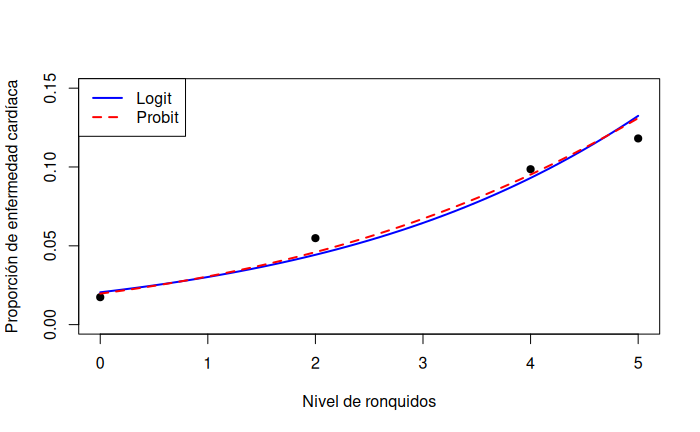
\includegraphics[scale=0.6]{Images/logit-probit-p02.png}\par
    \vspace{1cm}
    {\textit{\bfseries\huge Centro de Investigación en Matemáticas}\par}
    \vspace{0.5cm}
    {\large Maestría en Cómputo Estadístico\par}
    % {\large Ciencia de Datos\par} % opcional
    \vspace{1cm}
\end{center}

% Profesores y fecha
\begin{center} \large
    {\emph{\textbf{Catedráticos:}}}\\
    \large ME. José Ramón Domínguez Molina\par
    \large Dr. Rodrigo Macías Paéz\par
    \vspace{0.3cm}
    \large \today
\end{center}

\end{titlepage}


\restoregeometry%
\clearpage

%%%%%%%%%%%%%%%%%%%%%%%%%%%%%%%%%%%%%%%%%%%%%%
%%%        Tabla de Contenidos             %%%
%%%%%%%%%%%%%%%%%%%%%%%%%%%%%%%%%%%%%%%%%%%%%%
\hypertarget{MyToc}{}
\tableofcontents
\addtocontents{toc}{~\hfill\textbf{Página}\par}

%%%%%%%%%%%%%%%%%%%%%
%% Problemas      %%%
%%%%%%%%%%%%%%%%%%%%%
\newpage
%%%%%%%%%%%%%%%%%%%%%%%%%%%%%%%%%%%%%%%%%%%%%%%%%%%%%%%%%%%%%%%%
%%%%%%%%%%%%%%%%%%%%%%%%%%%%%%%%%%%%%%%%%%%%%%%%%%%%%%%%%%%%%%%%
%%%%%%%%%%%%%%%%%%%%%%%%%% Enunciado %%%%%%%%%%%%%%%%%%%%%%%%%%%

\begin{myblock}
\phantomsection\addcontentsline{toc}{section}{Ejercicio \#2 | Modelado de la Probabilidad de Enfermedad Cardíaca según el Nivel de Ronquido}
\section*{Ejercicio \#12| Modelado de la Probabilidad de Enfermedad Cardíaca según el Nivel de Ronquido}

Se tiene la siguiente tabla donde se eligen varios niveles de ronquidos y se ponen en relación con 
una enfermedad cardíaca. Se toman como puntuaciones relativas de ronquidos los valores $\{0, 2, 4, 5\}$.
\\

\begin{tabular}{lccc}
\hline
                & \multicolumn{2}{c}{\textbf{Enfermedad Cardiaca}} &                     \\ \cline{2-3}
\textbf{Ronquido}        & \textbf{SI}            & \textbf{NO}             & \textbf{Proporción de SI} \\ \hline
Nunca           & 24           & 1355          & 0.017               \\
Ocasional       & 35           & 603           & 0.055               \\
Casi cada noche & 21           & 192           & 0.099               \\
Cada noche      & 30           & 224           & 0.118               \\ \hline
\end{tabular}\\

Ajuste un modelo lineal generalizado logit y probit (investigar sobre el link probit), para analizar 
si existe una relación entre los roqnuidos y la posibilidad de tener enfermedad cardiaca. 

\end{myblock}

%%%%%%%%%%%%%%%%%%%%%%%%%%%%%%%%%%%%%%%%%%%%%%%%%%%%%%%%%%%%%%%%
%%%%%%%%%%%%%%%%%%%%%%%%%%%%%%%%%%%%%%%%%%%%%%%%%%%%%%%%%%%%%%%%

\subsection{Teoría}

Lo que queremos hacer en este problema es modelar la probabilidad de una enfermedad cardiaca en función 
del nivel de ronquidos $x_i$, definidos de manera ordinal: $\{0,2,4,5\}$. La probabilidad se modela como
$p_i = Pr(Y=1 | x_i)$. Como nuestra respuesta es binaria, i.e. tenemos conteos de éxito o fracaso por 
categoría, usaremos un GLM binomial con un enlace que mapea de (0,1) a $\mathbb{R}$. De ese modo 
podremmos comparar los dos enlaces estándar: logit y probit. 

Tenemos nuestros datos agrupados entre ``sí'' y ``no''. Para cada fila $i$, tenemos:

\[
    Y_i \sim \text{Binomial}(n_i, p_i) \;\;\;\;\;\; \text{con} \;\; y_i = \text{sí} \;\; \& \;\; n_i - y_i = \text{no}
\]

Por lo que nuestro modelo lineal generalizado queda como:

\[
    g(p_i) = \eta_i = \beta_0 + \beta_1 x_i
\]

Donde $g(\cdot)$ es el enlace. Por lo tanto, para la parte del logit, tenemos:

\[
    g(p) = \text{logit}(p) = \text{log}(\frac{p}{1-p})
\]

Entonces:

\[
    \text{log}(\frac{p}{1-p}) = \beta_0 + \beta_1 x_i \;\;\;\;\; => \;\;\;\;\; p_i = \frac{\text{exp}(\beta_0 + \beta_1 x_i)}{1 + \text{exp}(\beta_0 + \beta_1 x_i)}
\]

Esto nos está indicando que un cambio en $\Delta x$ multiplica los odds por $\exp(\beta_1 \Delta x)$, y 
en particular el odds ratio por unidad de $x$ es $\exp(\beta_1)$.

Ahora, en cuanto al enlace probit, tenemos:

\[
    g(p) = \phi^{-1}(p)
\]

Donde $\phi$ es la CDF Normal estándar, tal que tenemos un modleo de variable latente:

\[
    Z_i = \beta_0 + \beta_1 x_i + \epsilon_i \;\;\;\;\; \epsilon_i \sim \mathcal{N}(0,1) \;\;\;\;\; Y_i = 1\{Z_i > 0\} \;\; => \;\; p_i = \phi(\beta_0+\beta_1 + x_i)
\]

Entonces, para datos agrupados, tenemos una estimación de la log-verosimilitud de la forma:

\[
    \ell(\beta) = \sum_{i} \big[ y_i \text{log}(p_i) + (n_i - y_i) \text{log}(1-p_i) \big]
\]

Con $p_i$ como función de $\eta_i$ via el enlace. Así, se maximiza y los errores estándar provienen
de l amatriz de información observada. 

Además, tanto logit como probit producen curvas sigmoides muy similares. Las pendientes de ambas se
relacionan aproximadamente por un factor de escala:

\[
    \beta_{\text{logit}} \approx 1.7 \times \beta_{\text{probit}}
\]

De este modo, el modleo lineal generalizado aprende d euna sigmoide $p(x)$ que crece si $\beta_1 > 0$, 
i.e. con el nivel de ronquidos. 


%%%%%%%%%%%%%%%%%%%%%%%%%%%%%%%%%%%%%%%%%%%%%%%%%%%%%%%%%%%%%%%%%%%%%%%%%%%%
%%%%%%%%%%%%%%%%%%%%%%%%%%%%%%%%%%%%%%%%%%%%%%%%%%%%%%%%%%%%%%%%%%%%%%%%%%%%

\subsection{Resultados}

Tras ajustar los modelos de GLM binomiales a nuestros datos agrupados, los casos negativos o positivos
de enfermedad cardíaca por nivel de ronquidos, se compararon os enlaces logit y probit mediante AIC y 
deviance. Podemos visualizar el resultado en la figura \ref{fig:logit-probit-02}, mostrada a continuación.

\begin{figure}[h!]
    \centering
    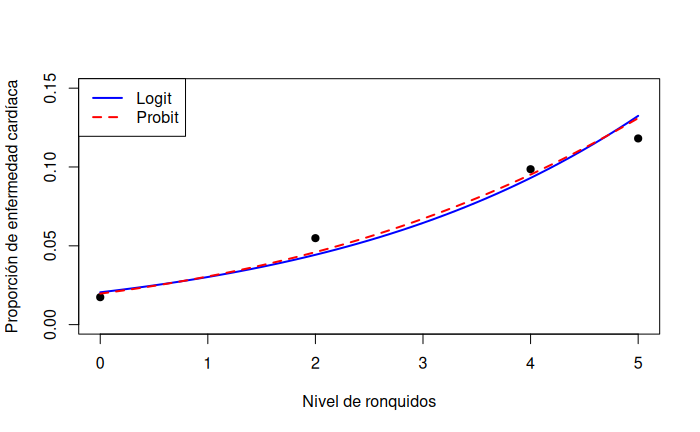
\includegraphics[width=0.7\linewidth]{Images/logit-probit-p02.png}
    \caption{Modelo logit vs. probit.}
    \label{fig:logit-probit-02}
\end{figure}

El cálculo propuesto encontró una asociación positiva y altamente significativa entre ronquidos y enfermedades
cardíacas con un $p-value < 10^{-6}$. En el modelo logit, tenemos un coeficiente de pendiente $\hat{\beta}_1 \approx 0.397$.
En cuanto al odds ratio por unidad en nuestra escala de roqnuidos, tenemos un valor de 1.49 con IC95\% $\approx [1.35, 1.64]$. 
Ahora, hablando del modleo probit, tenemos una pendiente de $\hat{\beta}_1 \approx 0.188$. Lo anterior 
confirma quye tenemos una misma tendencia, pues las magnitudes solo difieren un poco en escala. 

La diferencia por comparación de ajustes es $\text{AIC}(\text{logit} = 27.06)$ y $\text{AIC}(\text{probit} = 26.12)$. Tenemos
una discrepancia muy pequeña de apenas $\Delta \text{AIC} \approx 0.94$, por lo que ambos modelos se 
pueden considerar como equivalentes. 

La probabilidades predichas siguen de cerca las proporciones observadas, con subestimación leve en 
el nivel de roqnuidos 2 y sobreestimación ligera en el nivel 5. Además, un incremento de una unidad
en la escala de roqnuidos eleva la probabilidad de enfermedad cardiaca en un rango aproximado de 1.3 a 1.5
puntos porcentuales, dpeendiendo del nivel de referencia. 

De todo lo anterior, podeos llegar a la conclusión de que hay evidencia robusta de que a mayor frecuencia
de ronquidos, mayor es la probabilidad de presentar enfermedades cardíacas. Tanto el modleo logit como 
el modelo probit describen de manera adecuada el patrón de crecimiento, aunque el probit demuestra un ajuste
ligeramente mejor. Sin embargo, la diferencia entre ambos es muy pequeña. Quizás para casos médicos, es 
relevante escoger los modelos con mejor ajuste, aunque sea minimo, debido a la naturaleza del sector 
salud, donde justo la salud de los pacientes está en juego. 

%%%%%%%%%%%%%%%%%%%%%%%%%%%%%%%%%%%%%%%%%%%%%%%%%%%%%%%%%%%%%%%%%%%%%%%%%%%%
%%%%%%%%%%%%%%%%%%%%%%%%%%%%%%%%%%%%%%%%%%%%%%%%%%%%%%%%%%%%%%%%%%%%%%%%%%%%

%\subsection{Conclusiones}

%%%%%%%%%%%%%%%%%%%%%%%%%%%%%%%%%%%%%%%%%%%%%%%%%%%%%%%%%%%%%%%%%%%%%%%%%%%%
%%%%%%%%%%%%%%%%%%%%%%%%%%%%%%%%%%%%%%%%%%%%%%%%%%%%%%%%%%%%%%%%%%%%%%%%%%%%


\subsection{Código}

\begin{lstlisting}[caption={Modelos Logit y Probit para Enfermedad Cardiaca}, label={lst:glm_r}]
# Carga de datos
ronquidos <- c(0, 2, 4, 5)
si        <- c(24, 35, 21, 30)
no        <- c(1355, 603, 192, 224)
datos     <- data.frame(ronquidos = ronquidos, si = si, no = no)

# Ajuste de modelos GLM
modelo_logit  <- glm(cbind(si, no) ~ ronquidos, family = binomial(link = "logit"), data = datos)
modelo_probit <- glm(cbind(si, no) ~ ronquidos, family = binomial(link = "probit"), data = datos)

# Resumenes y comparacion
summary(modelo_logit)
summary(modelo_probit)
AIC(modelo_logit, modelo_probit)

# Predicciones para graficar
ronq_seq    <- seq(0, 5, by = 0.1)
pred_logit  <- predict(modelo_logit, newdata = data.frame(ronquidos = ronq_seq), type = "response")
pred_probit <- predict(modelo_probit, newdata = data.frame(ronquidos = ronq_seq), type = "response")

# Grafico comparativo
plot(ronquidos, si / (si + no), pch = 19, ylim = c(0, 0.15),
     xlab = "Nivel de ronquidos", ylab = "Proporcion de enfermedad cardiaca")
lines(ronq_seq, pred_logit, col = "blue", lwd = 2)
lines(ronq_seq, pred_probit, col = "red", lwd = 2, lty = 2)
legend("topleft", legend = c("Logit", "Probit"), col = c("blue", "red"), lty = c(1,2))
\end{lstlisting}

\subsection{Resumen de código}

\begin{itemize}
    \item \textbf{Datos:} Se cargan los datos en un \texttt{data.frame} que contiene los conteos de respuestas (\texttt{si}, \texttt{no}) y la variable predictora (\texttt{ronquidos}).

    \item \textbf{Modelos:} Se ajustan modelos lineales generalizados (\texttt{glm}) con la familia \texttt{binomial}, usando \texttt{link = "logit"} para la regresión logística y \texttt{link = "probit"} para el modelo probit. La respuesta se especifica para datos agrupados mediante \texttt{cbind(éxitos, fracasos)}.

    \item \textbf{Análisis:} Se utiliza \texttt{summary()} para obtener estimadores, errores estándar, estadísticos z y valores p. La calidad de ajuste entre modelos se compara con el Criterio de Información de Akaike usando \texttt{AIC()}.

    \item \textbf{Predicciones:} Se calculan las probabilidades predichas por cada modelo sobre una malla de valores de la variable \texttt{ronquidos} para facilitar la visualización.

    \item \textbf{Visualización:} Se genera un gráfico que muestra las proporciones observadas de los datos junto con las curvas de probabilidad predichas por los modelos logit y probit para una comparación visual del ajuste.
\end{itemize}


%%%%%%%%%%%%%%%%%%%%%%%%%%%%%%%%%%%%%%%%%%%%%%%%%%%%%%%%%%%%%%%%%%%%%%%%%%%%
%%%%%%%%%%%%%%%%%%%%%%%%%%%%%%%%%%%%%%%%%%%%%%%%%%%%%%%%%%%%%%%%%%%%%%%%%%%%

\clearpage





















\newpage
%%%%%%%%%%%%%%%%%%%%%%%%%%%%%%%%%%%%%%%%%%%%%%%%%%%%%%%%%%%%%%%%
%%%%%%%%%%%%%%%%%%%%%%%%%%%%%%%%%%%%%%%%%%%%%%%%%%%%%%%%%%%%%%%%
%%%%%%%%%%%%%%%%%%%%%%%%%% Enunciado %%%%%%%%%%%%%%%%%%%%%%%%%%%

\begin{myblock}
\phantomsection\addcontentsline{toc}{section}{Ejercicio \#3 | Análisis de Conteo de Parejas de Cangrejos Cacerola Mediante un GML Poisson}
\section*{Ejercicio \#3 | Análisis de Conteo de Parejas de Cangrejos Cacerola Mediante un GML Poisson}

Entre los cangrejos cacerola se sabe que cada hembra tiene un macho en su nido, pero puede tener más 
machos concubinos. Se considera que la variable respuesta es el número de concubinos y las variables
explicativas son: color, estado de la espina central, peso y anchura del caparazón.\\

\begin{center}
\begin{tabular}{ccccc}
\hline
\textbf{Color} & \textbf{Spine} & \textbf{Width} & \textbf{Satellite} & \textbf{Weight} \\
\hline
3 & 3 & 28.3 & 8 & 3050 \\
4 & 3 & 22.5 & 0 & 1550 \\
2 & 1 & 26.0 & 9 & 2300 \\
4 & 3 & 24.8 & 0 & 2100 \\
4 & 3 & 26.0 & 4 & 2600 \\
3 & 3 & 23.8 & 0 & 2100 \\
2 & 1 & 26.5 & 0 & 2350 \\
\hline
\end{tabular}
\end{center}

Realiza e interpreta los resultaados de ajustar un modelo lineal generalziado tipo Poisson. 

\end{myblock}

%%%%%%%%%%%%%%%%%%%%%%%%%%%%%%%%%%%%%%%%%%%%%%%%%%%%%%%%%%%%%%%%
%%%%%%%%%%%%%%%%%%%%%%%%%%%%%%%%%%%%%%%%%%%%%%%%%%%%%%%%%%%%%%%%

%%%%%%%%%%%%%%%%%%%%%%%%%%%%%%%%%%%%%%%%%%%%%%%%%%%%%%%%%%%%%%%%
%%%%%%%%%%%%%%%%%%%%%%%%%%%%%%%%%%%%%%%%%%%%%%%%%%%%%%%%%%%%%%%%

\subsection{Teoría}

En lo que respecta a Modelos Lineales Generalizados, el modelo Poisson constituye la herramienta
fundamental para analizar datos de conteo. En la pequeña base de datos que nos han otorgado, tenemos 
información sobre cangrejos cacelora, en la cual encontramos características físcias como el color, 
datos de la espina, anchura y peso. Estos datos fueron medidos de la hembra, es decir, se busca 
encontrar relación entre las características físicas de la hembra y la cantidad de concubinos que 
tiene. 

Este problema se compone de un avariable de respuesta $Y_i$, que es el número de concubinos (o machos satélite)
que acompañan a cada hembra. Tenemos un conteo de la siguiente forma:

\[
    Y_i \in \{0, 1, 2, ...., n\}
\]

Por ello, nuestro modelo a construir sera uno de Poisson, pues es el que mejor se acopla cuando tenemos 
una variable de interés con un conteo de eventos, tipo el número de clientes de una empresa, el número
de errores en un examen, o el número de miembros en un conjunto de animales. Recordemos que la distribución
Poisson con parámetro $\mu_i > 0$ tiene:

\[
    \text{P}(Y_i = y_i) = \frac{e^{-\mu_i} \mu_i^{y_i}}{y_i !} \;\;\;\;\; \text{con} \;\; y_i = 0,1,2,...
\]

En este caso, $\mu_i$ representa el número de concubinos de la cangrejo hembra. 

Ahora bien, en un GLM Poisson, tenemos la distribución de la familia exponencial $Y_i \sim \text{Poisson}(\mu_i)$. 
El enlace canico será:

\[
    g(\mu_i) = \log(\mu_i)
\]

Lo cual garantiza que $\mu_i > 0$. Así, el predictor lineal es:

\[
    \log(\mu_i) = \eta_i = \beta_0 + \beta_1 x_1 + \beta_2 x_2 + ...
\]

Finalmente, para nuestro caso, tenemos:

\[
    \log(\mu_i) = \beta_0 + \beta_1 \cdot \text{Color}_i + \beta_2 \cdot \text{Spine}_i + \beta_3 \cdot \text{Width}_i + \beta_4 \cdot \text{Weight}_i
\]

Podemos darle de inicio un poco de contexto sobre cómo se hará la interpretación. Bajo escala logarítmica,
tenemos:

\[
    \log(\mu_i) = \beta_0 + \beta_j x_{ij}
\] 

Exponenciando:

\[
    \mu_i = e^{\beta_0} \cdot e^{\beta_j x_{ij}}
\]

De ese modo, $e^{\beta_j}$ se interpreta como una razón de tasas de incidencia, o \textit{Incidence Rate Ratio} (IRR). Así:

\begin{itemize}
    \item Si $x_{ij}$ aumenta en una unidad, entonces $\mu_i$ se multiplica por $e^{\beta_j}$
    \item Si $e^{\beta_j} > 1$, entonces la variable incrementa el número esperado de concubinos.
    \item Si $e^{\beta_j} < 1$, entonces la variable reduce el número esperado de concubinos.
\end{itemize}

Por ejemplo, bajo este caso, suponiendo que tuvieramos un $\beta_3 = 0.25$. entonces $e^{0.25} \approx 1.28$
nos estaría diciendo que por cada aumento de una unidad en anchura, se espera un 28\% más de concubinos. Eso 
manteniendo las demás variables como constantes.

%%%%%%%%%%%%%%%%%%%%%%%%%%%%%%%%%%%%%%%%%%%%%%%%%%%%%%%%%%%%%%%%%%%%%%%%%%%
%%%%%%%%%%%%%%%%%%%%%%%%%%%%%%%%%%%%%%%%%%%%%%%%%%%%%%%%%%%%%%%%%%%%%%%%%%%

\subsection{Resultados}

\subsubsection{Anchura de Caparazón | \textit{Width}}

Para el caso de la varibale de anchura de caparazón, encontramos un IRR de 1.716 un un IC95\% de entre 1.28 y 2.29.
Es decir, por cada centímetro de anchura, se espera un incremento de concubinos del 71.6\%, o en otras
palabras, por cada centimetro, se multiplica el número de concubinos por 1.716 unidades. El Intercepto
tiene un valor de $2.16 \times 10^{-6}$. Entonces, podemos utilizar la media esperada para realizar predicciones,
esto se puede observar en el cuadro \ref{tab:width-capa}.\\

\begin{table}[h!]
    \centering
    \begin{tabular}{|c|c|}
        \hline
        \textbf{Anchura (cm)} & $\boldsymbol{\hat{\mu}}$ \textbf{(concubinos esperados)} \\
        \hline
        22.5 & 0.41 \\
        \hline
        24.0 & 0.92 \\
        \hline
        24.8 & 1.42 \\
        \hline
        26.0 & 2.71 \\
        \hline
        28.0 & 7.98 \\
        \hline
        28.3 & 9.38 \\
        \hline
    \end{tabular}
    \caption{Incremento de concubinos por cm.}
    \label{tab:width-capa}
\end{table}

Los resultados del cuadro anterior son consistentes con lo encontrado por la evidencia gráfica. La curvas
predicha nos indica que para anchiras pequeñas, de entre 22 y 24 centímetros, el valor esperado de
concubinos está entre 0 y 1. A partir de los 26 cm, la curva crece casi de manera exponencial,llegando a 
valores de 5 hasta 9 concubinos esperados. Podemos argumentar entonces que hembras más grandes
pueden esperar tener una mayor cantidad de concubinos. 

\begin{figure}[h!]
    \centering
    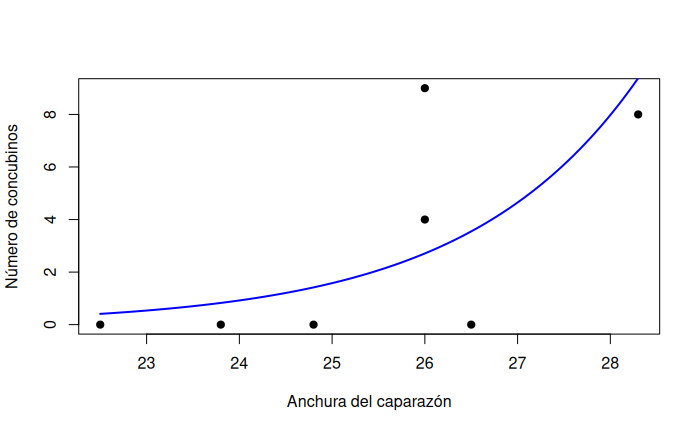
\includegraphics[width=0.7\linewidth]{Images/anchura-capa.png}
    \caption{Predicciones por anchura.}
    \label{fig:anchura-capa}
\end{figure}

Esto también es consistente con la biología de los cangrejos cacerola. Esta especie de animales presenta
dimorfismo sexual, es decir, hay una diferencia muy significativa entre el tamaño y la morfología de
los individuos hembra y macho. En el caso de los cangrejos cacerola, las hembras son mucho más grandes
que los machos, por lo que pueden ofrecer mayor protección y seguridad a una mayor cantidad de machos satélite.

Sin embargo, el crecimiento exponencial de concubinos seguramente debe tener un límite. Más datos serían
necesarios para comprender mejor cuál es la tendencia real. Aunque la evidencia es clara, mayor tamaño está
fuertemente correlacionado con mayor cantidad de concubinos. 

\subsubsection{Peso del Cangrejo | \textit{Weight}}

Para la variable peso, el modleo Poisson univariado arroja un IRR igual a 1.00194 por gramo, con IC95\%
entre 1.00088 y 1.00299. Es decir, por cada gramo adicional, el número de concubinos esperado se multiplica
por 1.00194. Quizás una lectura más práctica es que por cada 100 gramos, se espera un incrementro del
21.3\%.

El intercepto estimado es de 0.0253. Con este parámetro y la pendiente, podemo susar la media esperada $\hat{\mu}$
para hacer predicciones en pesos de interés, esto se resume como en el cuadro \ref{tab:peso-concubinos}.

\begin{table}[h!]
    \centering
    \begin{tabular}{|c|c|}
        \hline
        \textbf{Peso (g)} & \textbf{$\hat{\mu}$ (concubinos esperados)} \\
        \hline
        1550 & 0.51 \\
        \hline
        2100 & 1.46 \\
        \hline
        2350 & 2.37 \\
        \hline
        2600 & 3.85 \\
        \hline
        3050 & 9.19 \\
        \hline
    \end{tabular}
    \caption{Incremento de concubinos por peso}
    \label{tab:peso-concubinos}
\end{table}

Nuevamente, estos resultados son coherentes con la evidencia grfica: a bajos pesos, se esperan muy pocos 
concubinos, y al acercarnos a los 3,000 graos, la curva aumenta de forma marcada, alcanzando valores de
concubinos satélite de entre 4 y 9 miembros. Entonces, el peso también está fuertemente relacionado
con la cantidad de acompañantes de una hembra. Esto tiene mucho sentido, a mayor anchura, se puede 
esperar mayor peso, y a mayor peso mayor anchura.

\begin{figure}[h!]
    \centering
    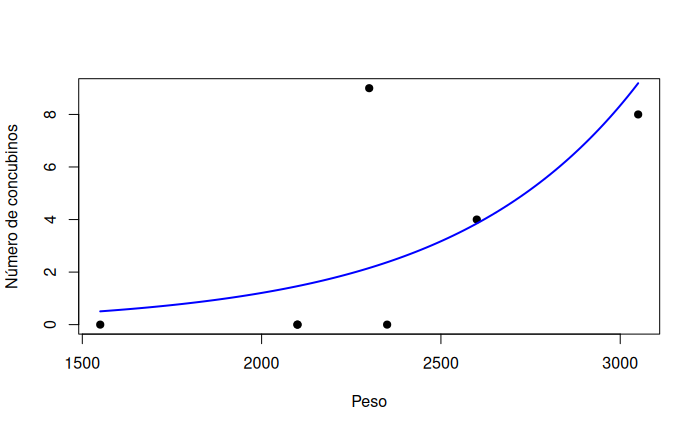
\includegraphics[width=0.7\linewidth]{Images/peso-capa.png}
    \caption{Predicciones por peso.}
    \label{fig:peso-capa}
\end{figure}

\subsubsection{Color del Caparazón | \textit{Color}}

Para la variable de color del caparazón, el modelo Poisson univariado arroja un IRR de 0.889 para el nivel
Color 3 respecto al nivel de referencia (Color 2), con un IC95\% entre 0.343 y 2.304. Esto indica que en
promedio, las hembras con coloración 3 presentan un 11\% menos concubinos que aquellas con coloración 2,
aunque el intervalo de confianza incluye el valor 1, por lo que no existe evidencia estadísticamente clara
de una diferencia entre estos grupos.

En el caso del nivel Color 4, el IRR estimado es de 0.296 con un IC95\% entre 0.091 y 0.962. Esto implica
que las hembras con coloración 4 tienen alrededor de un 70\% menos concubinos que las hembras con coloración 2.
En este caso, el límite superior del intervalo se encuentra por debajo de 1, lo que sugiere una posible
diferencia significativa, aunque debe tomarse con cautela debido al reducido tamaño muestral.

La media esperada $\hat{\mu}$ para cada nivel de color se resume en el cuadro \ref{tab:color-concubinos}.

\begin{table}[h!]
    \centering
    \begin{tabular}{|c|c|}
        \hline
        \textbf{Color} & \textbf{$\hat{\mu}$ (concubinos esperados)} \\
        \hline
        2 & 4.50 \\
        \hline
        3 & 4.00 \\
        \hline
        4 & 1.33 \\
        \hline
    \end{tabular}
    \caption{Número esperado de concubinos por nivel de color.}
    \label{tab:color-concubinos}
\end{table}

Estos resultados concuerdan con la evidencia gráfica: los colores 2 y 3 muestran medianas más altas, mientras
que el color 4 concentra valores bajos. Aunque los datos sugieren que la coloración puede estar asociada a
diferencias en el número de concubinos, la baja cantidad de observaciones por nivel impide una conclusión
firme.

\begin{figure}[h!]
    \centering
    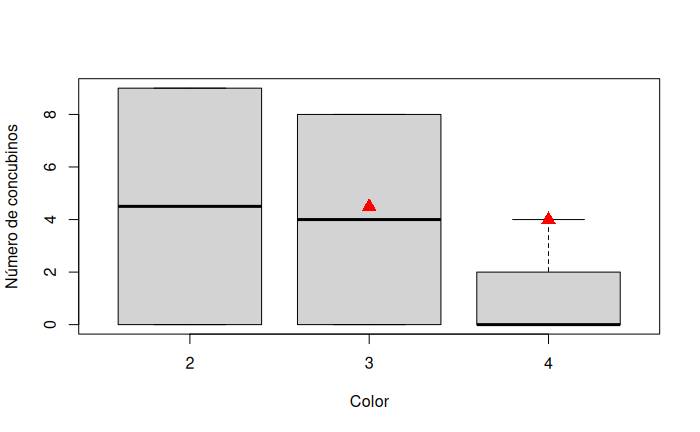
\includegraphics[width=0.7\linewidth]{Images/color-capa.png}
    \caption{Predicciones por color.}
    \label{fig:color-capa}
\end{figure}

\subsubsection{Estado de la Espina Central | \textit{Spine}}

Para la variable de estado de la espina central, el modelo Poisson univariado considera al nivel Spine 1
como referencia. El IRR estimado para Spine 3 es de 0.533 con un IC95\% entre 0.225 y 1.266. Esto sugiere
que las hembras con espina en estado 3 presentan aproximadamente un 47\% menos concubinos que aquellas con
espina en estado 1, aunque el intervalo de confianza incluye al 1, por lo que la evidencia no es suficiente
para concluir una diferencia estadísticamente significativa.

La media esperada $\hat{\mu}$ para cada nivel de espina se resume en el cuadro \ref{tab:spine-concubinos}.

\begin{table}[h!]
    \centering
    \begin{tabular}{|c|c|}
        \hline
        \textbf{Espina} & \textbf{$\hat{\mu}$ (concubinos esperados)} \\
        \hline
        1 & 4.50 \\
        \hline
        3 & 2.40 \\
        \hline
    \end{tabular}
    \caption{Número esperado de concubinos por nivel de espina.}
    \label{tab:spine-concubinos}
\end{table}

La gráfica comparativa muestra que el nivel 1 tiende a concentrar valores más altos y dispersos, mientras
que el nivel 3 se asocia con valores bajos a moderados. Sin embargo, nuevamente, la muestra es reducida y
los resultados deben considerarse exploratorios. Con un número mayor de observaciones sería posible evaluar
de manera más robusta si el estado de la espina central constituye un predictor significativo del número de
concubinos.

\begin{figure}[h!]
    \centering
    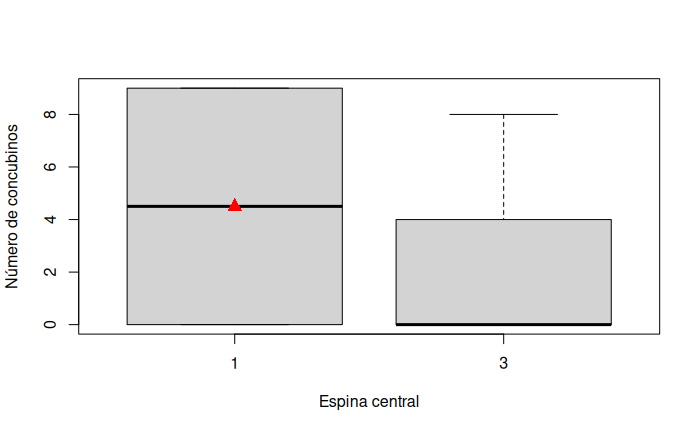
\includegraphics[width=0.7\linewidth]{Images/espina-capa.png}
    \caption{Predicciones por espina.}
    \label{fig:espina-capa}
\end{figure}

%%%%%%%%%%%%%%%%%%%%%%%%%%%%%%%%%%%%%%%%%%%%%%%%%%%%%%%%%%%%%%%%%%%%%%%%%%%
%%%%%%%%%%%%%%%%%%%%%%%%%%%%%%%%%%%%%%%%%%%%%%%%%%%%%%%%%%%%%%%%%%%%%%%%%%%

%%%%%%%%%%%%%%%%%%%%%%%%%%%%%%%%%%%%%%%%%%%%%%%%%%%%%%%%%%%%%%%%%%%%%%%%%%%
%%%%%%%%%%%%%%%%%%%%%%%%%%%%%%%%%%%%%%%%%%%%%%%%%%%%%%%%%%%%%%%%%%%%%%%%%%%

\subsection{Codigo}

\begin{lstlisting}[caption={Modelos de Regresion de Poisson para Cangrejos Cacerola}, label={lst:glm_crabs}]
# Carga y preparacion de datos
crabs <- data.frame(
  Color     = c(3,4,2,4,4,3,2),
  Spine     = c(3,3,1,3,3,3,1),
  Width     = c(28.3,22.5,26.0,24.8,26.0,23.8,26.5),
  Satellite = c(8,0,9,0,4,0,0),
  Weight    = c(3050,1550,2300,2100,2600,2100,2350)
)
crabs$Color <- factor(crabs$Color)
crabs$Spine <- factor(crabs$Spine)

# Funcion auxiliar para calcular IRR (Incidence Rate Ratios)
get_IRR <- function(model){
  ci <- confint.default(model)
  exp(cbind(Estimate = coef(model), ci))
}

# 1) Modelo con Width
m_width <- glm(Satellite ~ Width, data = crabs, family = poisson)
get_IRR(m_width)
newd_w <- data.frame(Width = seq(min(crabs$Width), max(crabs$Width), length.out = 100))
newd_w$mu_hat <- predict(m_width, newdata = newd_w, type="response")
plot(Satellite ~ Width, data = crabs, pch=19,
     xlab="Anchura del caparazon", ylab="Numero de concubinos")
lines(newd_w$Width, newd_w$mu_hat, col="blue", lwd=2)

# 2) Modelo con Weight
m_weight <- glm(Satellite ~ Weight, data = crabs, family = poisson)
get_IRR(m_weight)
newd_wt <- data.frame(Weight = seq(min(crabs$Weight), max(crabs$Weight), length.out = 100))
newd_wt$mu_hat <- predict(m_weight, newdata = newd_wt, type="response")
plot(Satellite ~ Weight, data = crabs, pch=19,
     xlab="Peso", ylab="Numero de concubinos")
lines(newd_wt$Weight, newd_wt$mu_hat, col="blue", lwd=2)
\end{lstlisting}

\subsection{Resumen de codigo}

\begin{itemize}
    \item \textbf{Datos:} Se cargan los datos de los cangrejos en un \texttt{data.frame}. Las variables \texttt{Color} y \texttt{Spine} se convierten a factores para su correcto tratamiento en los modelos.

    \item \textbf{Modelos:} Se ajustan múltiples modelos lineales generalizados univariados con \texttt{glm}, utilizando la familia \texttt{poisson} con enlace logarítmico, que es adecuado para datos de conteo. Cada modelo evalúa la relación entre el número de concubinos (\texttt{Satellite}) y una única variable predictora (ej. \texttt{Width}, \texttt{Weight}).

    \item \textbf{Análisis:} Se define una función auxiliar, \texttt{get\_IRR}, para calcular los \textit{Incidence Rate Ratios} (IRR) y sus intervalos de confianza. Estos valores se utilizan para interpretar el efecto multiplicativo de cada predictor sobre el número esperado de concubinos.

    \item \textbf{Predicciones:} Para las variables continuas (\texttt{Width}, \texttt{Weight}), se generan predicciones del número esperado de concubinos sobre una secuencia de valores, permitiendo trazar una curva de ajuste suave.

    \item \textbf{Visualización:} Se crea un gráfico para cada modelo, mostrando los datos observados (puntos) y la relación predicha por el modelo (línea o puntos de predicción). Esto permite una comparación visual del ajuste del modelo a los datos.
\end{itemize}

\clearpage










\newpage
%%%%%%%%%%%%%%%%%%%%%%%%%%%%%%%%%%%%%%%%%%%%%%%%%%%%%%%%%%%%%%%%
%%%%%%%%%%%%%%%%%%%%%%%%%%%%%%%%%%%%%%%%%%%%%%%%%%%%%%%%%%%%%%%%
%%%%%%%%%%%%%%%%%%%%%%%%%% Enunciado %%%%%%%%%%%%%%%%%%%%%%%%%%%

\begin{myblock}
\phantomsection\addcontentsline{toc}{section}{Ejercicio \#5 | Curvas ROC/AUC}
\section*{Ejercicio \#5 | Curvas ROC/AUC}

Construyan la curva ROC para el problema de daño coronario y su relación con la edad visto en la
clase 3 del curso. 

\end{myblock}

%%%%%%%%%%%%%%%%%%%%%%%%%%%%%%%%%%%%%%%%%%%%%%%%%%%%%%%%%%%%%%%%
%%%%%%%%%%%%%%%%%%%%%%%%%%%%%%%%%%%%%%%%%%%%%%%%%%%%%%%%%%%%%%%%

\subsection{Teoría}

    \subsubsection{Especificidad y Sensibilidad}

        Las curvas ROC, del acrónimo en inglés ``\textit{Receiver Operating Characteristic}'', es una herramienta
        bastante útil para la evaluación de clasificadores. Formalmente, dado un clasificador que produce scores
        continuos $S \in \mathbb{R}$, la curva ROC representa el conjunto de pares $(FPR(t), TPR(t))$ para
        todo $t \in \mathbb{R}$, donde $t$ es un umbral de decisión.

        Matemáticamente hablando, para una variable aleatoria continua $X$ que representa los scores y una variable
        indicadora $Y \in \{0,1\}$, que representa la clase verdadera, tenemos:

        \begin{itemize}
            \item $TPR(t) = P(X > t | Y = 1) = 1 - F_1(t)$
            \item $FPR(t) = P(X > t | Y = 0) = 1 - F_0(t)$
        \end{itemize}

        Donde $F_1$ y $F_0$ son las funciones de distribución acumulada condicionales de $X$ dado $Y = 1$ y
        $Y = 0$, respectivamente.  

        Ahora bien, el AUC, o Área Bajo la Curva, posee una elegante interpretación probabilística que fundamenta
        su utilidad como medida de desempeño: $\text{AUC} = P(S^+ > S^-)$. En este caso, $S^+$ y $S^-$ son scores
        independientes correspondientes a observaciones positivas y negativas, respectivamente. Esta formulación
        establece que el AUC equivale a la probabilidad de que el clasificador asigne un score mayor a una observación
        positiva elegida aleatoriamente que a una negativa aleatoriamente. 

        Hablando de los ejes, el Eje X se refiere a los \textit{False Positive Rate}, o FPR:

        \[
            \text{FPR} = \frac{\text{FP}}{\text{FP + TN}} = 1 - \text{Especificidad}
        \]

        Este eje representa la fracción de negativos que el modelo clasifica erróneamente como positivos. 

        En cuanto al eje Y, se trata del \textit{True Positive Rate} o TPR, y se define como:

        \[
            \text{TPR} = \frac{\text{TP}}{\text{TP + FN}} = \text{Sensibilidad}
        \]

        Representa la fracción de positivos correctamente identificados por el modelo. 

        Creo que es importante recordar lo que son Sensibilidad y Especificidad. La sensibilidad o \textit{recall}, 
        es una métrica que se encarga de medir la capacidad delk modelo para identificar correctamente los verdaderos
        positivos. Es fundamental en contextos donde los falsos negativos son costosos, como en aplicaciones de medicina
        o algo del apartado legal. En cuanto a la Especificidad, esta mide la capacida ddel modelo de identificar
        de manera correcta los verdaderos negativo. Es de vital importancia para cuando los falsos positivos 
        son costosos, quizás para la aprobación de créditos. 

        De ese modo, cada punto de la curva representa un posible umbral de decisión. Cuando el umbrla es
        muy bajo, el modelo es demasiado flexible y clasifica en su mayoría como positivo, i.e. cuando TPR y FPR son altos.
        Cuando el umbral es muy alto, el modelo es muy rígido y clasidica casi todo como negativo, Esto es cuando TPR y FPR son bajos. 

        La recta que cruza por la identidad en las curvas ROC es la ``línea del azar''. La línea diagonal que
        une (0,0) con (1,1) corresponde a lo que sería un clasificador aleatorio, uno sin la capacidad de discernir. Cuando
        el modelo está sobr esta línea, entonces su desempeño no se puede distinguir del azar. Cuanto ms arriba 
        de la línea se encuentre la curva, mejor será la discriminación.

        Una de las desventajas de la curva ROC es que no es sensible al desbalance de clases. Para cuando hay
        prevalencia de desbalanceo de clases, se prefiere utilizar la curva \textit{Precision-Recall} (PR). Para
        la evaluación de modelos, la ROC es bastante útil para comparar de forma global.

    \subsubsection{Estadístico de Youden}

        El estadístico de Youden, también conocido como índice J, fue introducido en 1950 por W.J. Youden como
        una medida resumen de la efectividad de una prueba diagnóstica. Se define como:

        \[
            J = \text{Sensibilidad} + \text{Especificidad} - 1
        \]

        El rango del índice es, naturalemnte, $-1 \leq J \leq 1$. Sin embargo, en aplicaciones prácticas, 
        se acota a $0 \leq J \leq 1$, ya que la sensibilidad y especificidad son no negativas. En el caso de
        la curva ROC, tenemos que la Sensibilidad es TPR y que 1 - Especificidad es FPR. Entonces:

        \[
            J = TPR - FPR
        \]

        Por lo tanto, $J$ mide la distancia vertical máxima entre la curva ROC y la diagonal de azar.

        \begin{itemize}
            \item $J = 0$ el modelo no discrimina, i.e. estaríamos hablando a un clasificador aleatorio.
            \item $J = 1$ el modelo clasifica de manera perfecta, i.e. la sensibilidad y especificidad son ambos 1.
            \item Valore sintermedios reflejan la capacidad de la prueba de mejorar sobre el azar. 
        \end{itemize}

        Cuando un modelo produce un puntaje o probabilidad, se necesit aun umbral de decisión para clasificar. El
        umbral óptimo de Youden se define como aquel que maximiza $J$:

        \[
            \hat{t} = \text{arg} \max_t \bigg(\text{Sensibilidad}(t) + \text{Especificidad}(t) - 1\bigg)
        \]

        Este pubnto corresponde al punto de la curva ROC más alejado de la diagonal del azar. 

    \subsubsection{Estadístico Kolmogorov-Smirnov (KS)}

    Este estadístico proviene originalmente de la prueba KS para comparar dos distribuciones acumuladas. En
    su forma general:

    \[
        D = \sup_x |F_n(x) - F(x)|
    \]

    Es la máxima diferencia entre una función de distribución empírica y una distribución teórica. En
    clasificación binaria, se adapta para medir la separación enter las distribuciones de puntajes (o probabilidades)
    de las dos clases. 

    La interpretación probabilística del KS mide cuán bien el modelo separa las distribuciones de scores
    entre positivos y negativos. Geométricamente, se demuestra que:

    \[
        KS = \max_t |TPR(t) - FPR(t)|
    \]

    Donde $t$ es un umbral de decisión. Es decir, $KS$ es la máxima diferencia vertical entre la curva ROC
    y la diagonal de azar. Esto es identico al de Youden solo cuando $TPR \geq FPR$. 

    \begin{itemize}
        \item KS = 0 nos dice que no hay discriminación, las distribuciones son idénticas.
        \item KS = 1 nos dice que la separación es perfecta, sin solapamientos entre positivos y negativos.
        \item Los valores intermedios reflejan distintos niveles de discriminación.
    \end{itemize}

\subsubsection{Distancia al punto (0,1)}

En el espacio ROC, el punto ideal para un clasificador perfecto es (0,1), pues se traduce en FPR = 0, i.e. ningún
falso positivo, y TPR = 1, i.e. todos los positivos identificados correctamente. Minimizar la distancia a 
ese punto significa encontrar el mejor compromiso entre reducir los falsos positivos y aumentar los verdaderos positivos. A 
diferencia del índice Youden, este midel al distancia euclidiana absoluta ideal. 


%%%%%%%%%%%%%%%%%%%%%%%%%%%%%%%%%%%%%%%%%%%%%%%%%%%%%%%%%%%%%%%%
%%%%%%%%%%%%%%%%%%%%%%%%%%%%%%%%%%%%%%%%%%%%%%%%%%%%%%%%%%%%%%%%

\subsection{Resultados}
\textcolor{red}{
En este caso, grafiqué dos curvas ROC. Al final me di cuenta de que fue redundante, porque este tipo de visualizaciones para problemas de clasificación binaria no necesitan mostrar
la aproximación cuando se toma a 1 o a 0 como la clase positiva. Obtener los dos gráficos y obtener
sus estadísticos es redundante. Sin embargo se ven bonitas las gráficas.}
\clearpage

    \subsubsection{Estadístico de Youden \& Kolmogorov-Smirnov}

        \begin{figure}[h!]
            \centering
            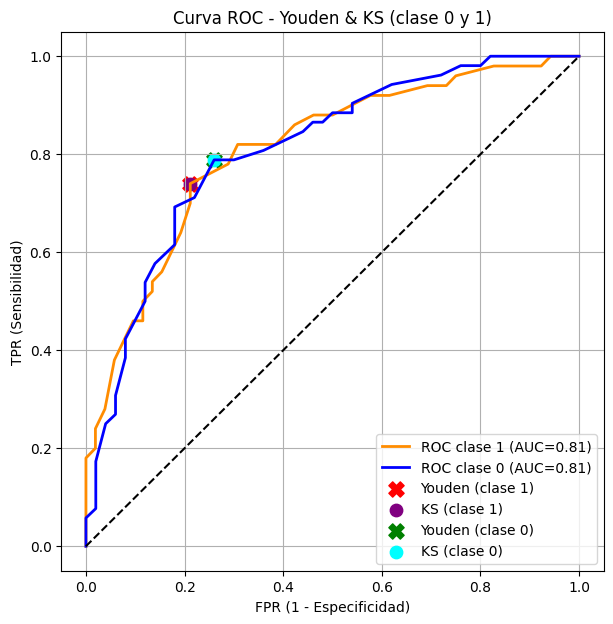
\includegraphics[width=0.7\linewidth]{Images/youden-ks-roc.png}
            \caption{Curva AUC/ROC con los estadísticos de Youden \& KS fijos en el mismo lugar.}
            \label{fig:youden-ks-roc}
        \end{figure}
        \clearpage

    \subsubsection{Punto (0,1) geométrico.}

        \begin{figure}[h!]
            \centering
            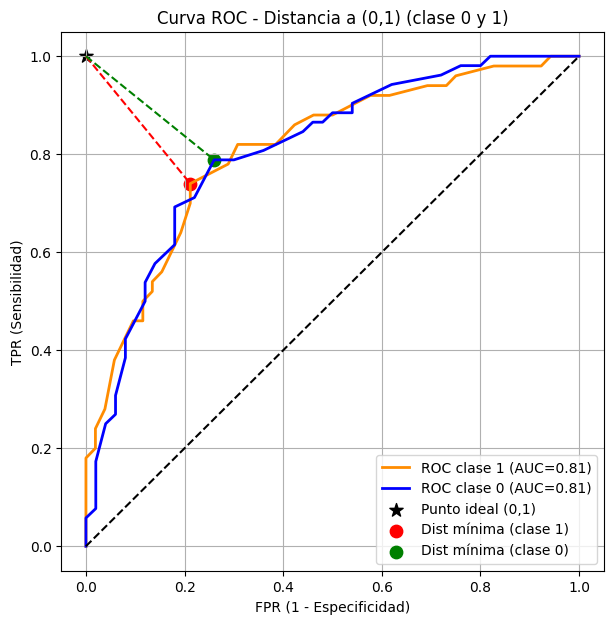
\includegraphics[width=0.7\linewidth]{Images/dist-geom-roc.png}
            \caption{Curva AUC/ROC con los estadísticos geométricos en el mismo lugar que el de Youden \& KS.}
            \label{fig:geom-roc}
        \end{figure}

    \subsubsection{Discusión de resultados}

        Para nuestro caso, nos encontramos con que el estadístico de Youden, el de Kolmogorov-Smirnov y 
        la distancia del máximo de la ROC hacia el punto (0,1) coinciden por completo. Es decir, existe
        un punto óptimo único dentro de la curva, de tal modo que se maximiza la capacidad del modelo 
        bajo el mismo umbral. 

        Recordemos que el índice de Youden maximiza la suma de la sensibilidad y especificidad. Esto es,
        equivale a cuando encontramos el punto donde la diferencia entre la tasa de verdaderos positivos, y la
        de falsos positivos es máxima, i.e. el punto más alejado de la recta del azar. El estadístico de
        KS maximiza la separación entre las distribuciones de scores de las clases positiva y negativa. En
        cuanto a la distancia al punto (0,1), este minimiza la distancia euclidiana al punto ideal donde TPR = 1 
        y FPR = 0, mientras más bajo el valor, más cerca de la mejor clasificación está nuestro modelo. 

        Que los puntos coincidan nos está diciendo que existe un punto de operación óptimo. Entonces tenemos
        un umbrla que ofrece un rendimiento consistente y robusto. A pesar de que graficamos dos ROC, una para
        cuando la clase 1 es positiva y otra para cuando la 0 es positiva (redundante por ser un clasificador
        biomial), concentremonos en la clase 1 como la positiva. Cuando clase 1 es positiva, el umbral óptimo está en 0.524m con un accuracy de 0.765 y un F1-score de 
        0.755. 

        Finalmente, la coincidencia de estadísticos nos facilita la elección del umbral en la práctica, ya
        que no hay conflicto entre los criterios. Es importante recordar que el umbral es un valor que nos 
        permite configurar qué tan flexible será nuestro modelo. Por ejemplo, si la probabilidad < umbral, entonces
        se toma como clase negativa, si la probabilidad es $/geq$ umbral, entonces tomamos clase positiva.
        
        Si hacemo suna analogía, un umbral de 0.3, dejamos que varios falsos positivos sean clasificados de manera
        incorrecta. Si tomamos un umbral de 0.8, dejamos que algunos verdaderos positivos sean mal clasificados. 
        

%%%%%%%%%%%%%%%%%%%%%%%%%%%%%%%%%%%%%%%%%%%%%%%%%%%%%%%%%%%%%%%%
%%%%%%%%%%%%%%%%%%%%%%%%%%%%%%%%%%%%%%%%%%%%%%%%%%%%%%%%%%%%%%%%

\subsection{Código}

    \begin{lstlisting}[caption={Analisis de Curva ROC para Clasificacion Logistica}, label={lst:roc_analysis_py}]
    # --- Ajuste del modelo y funcion auxiliar ---
    # Modelo logistico
    logit = LogisticRegression(solver="lbfgs")
    logit.fit(edad.reshape(-1, 1), coro)
    phat = logit.predict_proba(X)[:, 1] # Probabilidad de la clase 1

    # Funcion que calcula metricas ROC y puntos de corte optimos
    def compute_metrics(y_true, scores, positive_label=1):
        if positive_label == 0: # Invierte para analizar la clase 0
            y_true, scores = 1 - y_true, 1 - scores

        fpr, tpr, thresholds = roc_curve(y_true, scores)
        roc_auc = auc(fpr, tpr)

        # Puntos de corte optimos
        youden_idx = np.argmax(tpr - fpr)
        ks_idx = np.argmax(np.abs(tpr - fpr))
        dist_idx = np.argmin(np.sqrt(fpr**2 + (tpr - 1)**2))

        # Resultados en puntos optimos
        results = {}
        for name, thr in [("Youden", thresholds[youden_idx]),
                        ("KS", thresholds[ks_idx]),
                        ("Dist", thresholds[dist_idx])]:
            y_pred = (scores >= thr).astype(int)
            acc = accuracy_score(y_true, y_pred)
            f1 = f1_score(y_true, y_pred)
            results[name] = (thr, acc, f1)

        return fpr, tpr, roc_auc, youden_idx, ks_idx, dist_idx, results

    # --- Calculo y visualizacion ---
    # Metricas para ambas clases
    fpr1, tpr1, auc1, y_idx1, ks_idx1, d_idx1, res1 = compute_metrics(y, phat, 1)
    fpr0, tpr0, auc0, y_idx0, ks_idx0, d_idx0, res0 = compute_metrics(y, phat, 0)

    # Se grafica con matplotlib

    # Imprimimos metricas
    \end{lstlisting}


\subsection{Resumen de codigo}

\begin{itemize}
    \item \textbf{Modelo y Predicciones:} Se ajusta un modelo de regresion logistica utilizando la edad como predictor. Posteriormente, se calculan las probabilidades predichas (\texttt{phat}) para la clase positiva (1).

    \item \textbf{Funcion de Metricas:} Se define una funcion, \texttt{compute\_metrics}, que es el nucleo del analisis. Esta funcion calcula la curva ROC y el area bajo la curva (AUC). Ademas, identifica los umbrales de decision optimos basados en tres criterios distintos:
    \begin{itemize}
        \item El indice de Youden (maximizando la diferencia TPR - FPR).
        \item La estadistica de Kolmogorov-Smirnov (KS) (maximizando la diferencia absoluta |TPR - FPR|).
        \item La distancia minima al punto ideal (0,1) en el grafico ROC.
    \end{itemize}
    Para cada umbral optimo, la funcion tambien calcula la exactitud (accuracy) y la puntuacion F1.

    \item \textbf{Analisis por Clase:} La funcion de metricas se aplica dos veces para evaluar el rendimiento del clasificador tanto para la clase 1 (positiva) como para la clase 0 (negativa). Para la clase 0, se invierten las etiquetas y las probabilidades.

    \item \textbf{Visualizacion:} Se generan dos graficos de la curva ROC para comparar el rendimiento de ambas clases. El primer grafico resalta los puntos optimos segun Youden y KS, mientras que el segundo resalta el punto optimo basado en la distancia minima a (0,1).

    \item \textbf{Reporte:} Finalmente, se imprime un resumen en la consola que muestra el valor del umbral, la exactitud y la puntuacion F1 para cada uno de los tres criterios de optimizacion, detallando los resultados para ambas clases.
\end{itemize}

%%%%%%%%%%%%%%%%%%%%%%%%%%%%%%%%%%%%%%%%%%%%%%%%%%%%%%%%%%%%%%%%
%%%%%%%%%%%%%%%%%%%%%%%%%%%%%%%%%%%%%%%%%%%%%%%%%%%%%%%%%%%%%%%%

%\subsection{Conclusiones}

%%%%%%%%%%%%%%%%%%%%%%%%%%%%%%%%%%%%%%%%%%%%%%%%%%%%%%%%%%%%%%%%
%%%%%%%%%%%%%%%%%%%%%%%%%%%%%%%%%%%%%%%%%%%%%%%%%%%%%%%%%%%%%%%%

\clearpage





\newpage
%%%%%%%%%%%%%%%%%%%%%%%%%%%%%%%%%%%%%%%%%%%%%%%%%%%%%%%%%%%%%%%%
%%%%%%%%%%%%%%%%%%%%%%%%%%%%%%%%%%%%%%%%%%%%%%%%%%%%%%%%%%%%%%%%
%%%%%%%%%%%%%%%%%%%%%%%%%% Enunciado %%%%%%%%%%%%%%%%%%%%%%%%%%%

\begin{myblock}
\phantomsection\addcontentsline{toc}{section}{Ejercicio \#7 | Seguros}
\section*{Ejercicio \#7 | Seguros}

Los datos dentrl del cuadro \ref{tab:seguros} son números $n$ de pólizas de seguros, y los correspondientes
numeros $y$ de reclamos (esto es, número de accidentes en los que se pidió el amparo de la poliza). La
variable \texttt{CAR} es una codificación de varias clases de carros, \texttt{EDAD} es la edad del 
titular de la póliza y \texttt{DIST} es el distrito donde vive el titular.

\textbf{(a)} Calcule la tasa de reclamos $\frac{y}{n}$ para cada categoría y grafique estas tasas contra 
las diferentes variables para tener una idea de los efectos principales. 

\end{myblock}

%%%%%%%%%%%%%%%%%%%%%%%%%%%%%%%%%%%%%%%%%%%%%%%%%%%%%%%%%%%%%%%%
%%%%%%%%%%%%%%%%%%%%%%%%%%%%%%%%%%%%%%%%%%%%%%%%%%%%%%%%%%%%%%%%

\begin{table}[h!]
    \centering
    \begin{tabular}{cc|cc|cc}
        \hline
        \textbf{CAR} & \textbf{EDAD} & \multicolumn{2}{c|}{\textbf{DIST = 0}} & \multicolumn{2}{c}{\textbf{DIST = 1}} \\
        & & \textbf{y} & \textbf{n} & \textbf{y} & \textbf{n} \\
        \hline
        1 & 1 & 65  & 317  & 2   & 20   \\
        1 & 2 & 65  & 476  & 5   & 33   \\
        1 & 3 & 52  & 486  & 4   & 40   \\
        1 & 4 & 310 & 3259 & 36  & 316  \\
        \hline
        2 & 1 & 98  & 486  & 7   & 31   \\
        2 & 2 & 159 & 1004 & 10  & 81   \\
        2 & 3 & 175 & 1355 & 22  & 122  \\
        2 & 4 & 877 & 7660 & 102 & 724  \\
        \hline
        3 & 1 & 41  & 223  & 5   & 18   \\
        3 & 2 & 117 & 539  & 7   & 39   \\
        3 & 3 & 137 & 697  & 16  & 68  \\
        3 & 4 & 477 & 3442 & 63  & 344  \\
        \hline
        4 & 1 & 11  & 40   & 0   & 3    \\
        4 & 2 & 35  & 148  & 6   & 16   \\
        4 & 3 & 39  & 214  & 8   & 25   \\
        4 & 4 & 167 & 1019 & 33  & 114  \\
        \hline
    \end{tabular}
    \caption{Numero de polizas (n) y reclamos (y) por tipo de carro, edad y distrito.}
    \label{tab:seguros}
\end{table}

%%%%%%%%%%%%%%%%%%%%%%%%%%%%%%%%%%%%%%%%%%%%%%%%%%%%%%%%%%%%%%%%
%%%%%%%%%%%%%%%%%%%%%%%%%%%%%%%%%%%%%%%%%%%%%%%%%%%%%%%%%%%%%%%%


Vamos a calcular la tasa de reclamos para cada celda de la tabla:

\[
    \text{tasa} = \frac{y}{n}
\]

Donde $y$ es el número de reclamos o accidentes reportados, y $n$ el número de pólizas. Esto nos da 
una medida de la frecuencia relativa de accidentes en cada categoría. Luego, graficaremos estas tasas 
contra las variables explicativas (\texttt{CAR}, \texttt{EDAD}, \texttt{DIST}) para visualizar los
efectos principales.  

La parte matemática formal quedaría como lo siguiente. Dado un dataset indexado por $i$ (combinaciones
de nuestras tres variables), definimos:

\[
    \hat{\pi}_i = \frac{y_i}{n_i} \;\;\;\;\; \text{con} \;\; 0 \leq \hat{pi}_i \leq 1
\]

La interpretación es que $\hat{pi}_i$ estima la probabilidad de reclamo para una póliza de la categoría $i$.

Básicamente, lo que haremos será construir nuestro dataframe en R, calcular la tasa creando una nueva
columna dentro del dataframe, a la cual podemos llamar \texttt{rate} y que esté definida por la tasa $\frac{y}{n}$.
De ese modo, graficamos cómo cambia la tasa acorde a cada variable (\texttt{CAR}, \texttt{EDAD}, \texttt{DIST}).

\subsubsection{Resultados (a)}

El gráfico de tasas específicas (Figura 1), muestra que en \texttt{DIST=0} las tasas de reclamo disminuyen
de manera consistentee a medida que aumenta la edad del titular, con diferencias clasras entre tipos de 
carro. En \texttt{DIST = 1}, el patrón es menos regular, aunque destaca un pico particularmente alto en 
\texttt{CAR=4} y \texttt{EDAD=2}, dejando entrever interacción entre variables. 

Ahora bien, podemos resumir los efectos promedio de cada variable, calculando las tasas agregadas ponderadas
por el número de pólizas, junto con intervalos de confianza binomiales. 

\begin{itemize}
    \item \textbf{CAR}: la tasa promedio aumenta de manera monótona desde \texttt{CAR=1} hasta \texttt{CAR=4}. 
    Esto indica que ciertos tipos de automóviles están asociados a mayor frecuencia de reclamos.
    \item \textbf{EDAD}: podemos notar que hay un gradiente pronnunciado negativo. Los titulares más jovenes,
    i.e. \texttt{EDAD=1} presentan tasas cercanas a 0.20, mientras que los mayores, referentes a \texttt{EDAD=4}
    alcanzan apenas 0.12. El patrón indica una disminución del riesgo de reclamo a mayor edad del titular, o conductor.
    \item \textbf{DIST}: en cuanto a los dos distritos, el distrito 1 presenta mayor tasa promedio que el 2. 
    mientras que el distrito 1 tienen 0.165 puntos, el segundo tiene 0.132. Esto puede ser un posible efecto
    de localización geográfica en el riesgo de los accidentes. 
\end{itemize}

Estos resultados no sindican que las características del automóvil, la edad del conductor y el distrito
de residencia son factores asociados de manera importante con la frecuencia de los reclamos. Las figuras
encontradas demuestran que los vehículos de categorías 3 y 4 muestran un riesgo considerablemente mayor 
a las otras. De igual forma, el riesgo de siniestros disminuye con la edad del conductor, esto hace un 
poco de sentido si tomamos en cuenta que los conductores jóvenes tienen menos experiencia al volante 
y pueden resultar un poco más temerarios al moemnto de tomar el carro. El efecto del distrito parece 
ser el de menor impacto. 

\begin{figure}[h!]
    \centering
    
    % --- Primera Fila ---
    \begin{subfigure}[b]{0.48\textwidth}
        \centering
        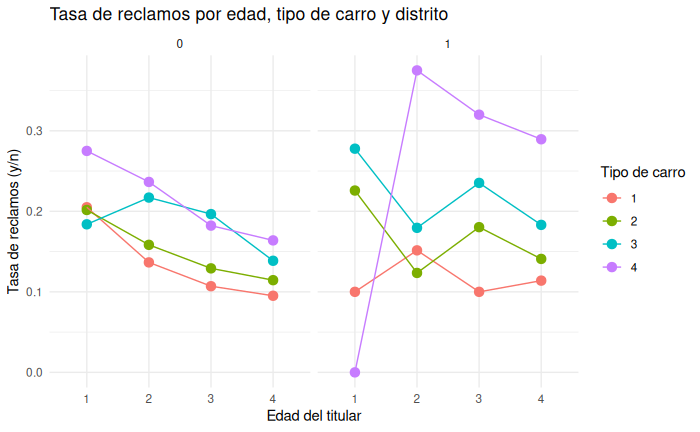
\includegraphics[width=\textwidth]{Images/tasa-reclamos-edad-titular.png}
        \caption{Tasa de las distintas variables.}
        \label{fig:img1}
    \end{subfigure}
    \hfill % Espacio horizontal entre las imágenes
    \begin{subfigure}[b]{0.48\textwidth}
        \centering
        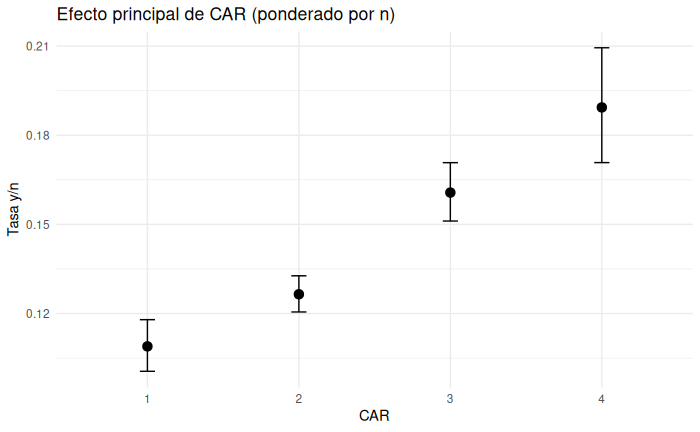
\includegraphics[width=\textwidth]{Images/CAR-seguros.png}
        \caption{Tasa vs. Carro.}
        \label{fig:img2}
    \end{subfigure}
    
    \vspace{0.5cm} % Espacio vertical entre las filas
    
    % --- Segunda Fila ---
    \begin{subfigure}[b]{0.48\textwidth}
        \centering
        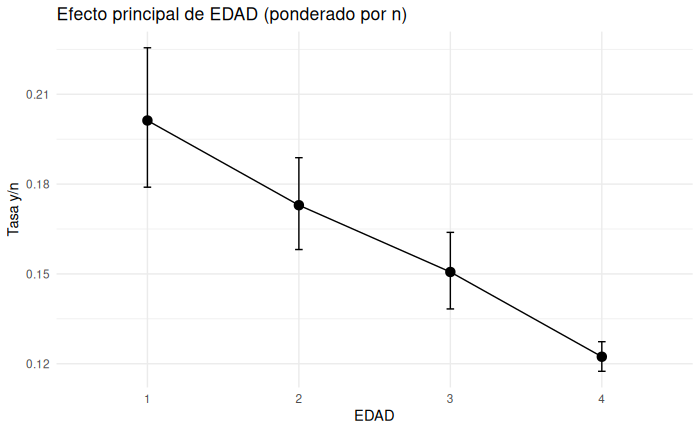
\includegraphics[width=\textwidth]{Images/EDAD-seguros.png}
        \caption{Tasa vs. Edad.}
        \label{fig:img3}
    \end{subfigure}
    \hfill % Espacio horizontal
    \begin{subfigure}[b]{0.48\textwidth}
        \centering
        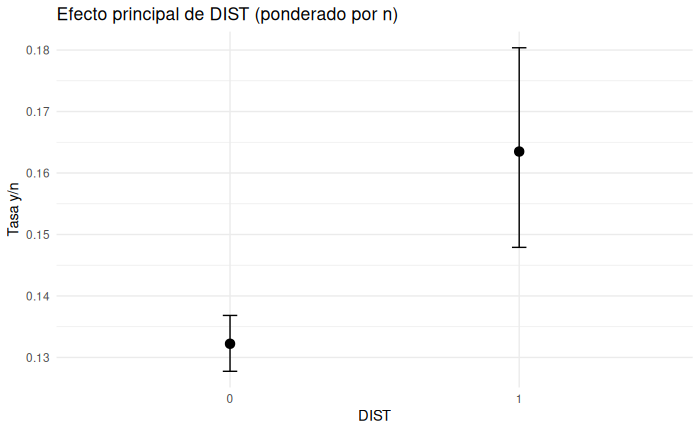
\includegraphics[width=\textwidth]{Images/DIST.png}
        \caption{Tasa vs. Distrito.}
        \label{fig:img4}
    \end{subfigure}
    
    \caption{Gráfica de las tasas vs. cada variable.}
    \label{fig:matriz_imagenes}
\end{figure}

%%%%%%%%%%%%%%%%%%%%%%%%%%%%%%%%%%%%%%%%%%%%%%%%%%%%%%%%%%%%%%%%%%%%%%%%%%%%%
%%%%%%%%%%%%%%%%%%%%%%%%%%%%%%%%%%%%%%%%%%%%%%%%%%%%%%%%%%%%%%%%%%%%%%%%%%%%%

\begin{myblock}
    
    \textbf{(b)} Ajusta un modelo de Poisson apropiado. 

\end{myblock}

\subsubsection{Modelo GLM Poisson}

Ajustamos un modelo GLM Poisson para los conteos $y_i$ con enlace log y \text{offset} $log(n_i)$:

\[
    y_i \sim Poisson(y_i) \;\;\;\;\; log(y_i) = log(n_i) + \beta_0 + \beta(\text{CAR}) + \beta(\text{EDAD}) + \beta(\text{DIST})
\]

De los tres modelos $(m_0 = 378.19, m_1 = 208.07, m_2 = 219.66)$, el modelo $m_1$ es el que tiene el AIC mínimo. 
La Binomial Negativa no mejora, por lo que el modelo final es Poisson con una combinación de las variables. 

\begin{table}[h!]
    \centering
    \caption{Resumen de IRR (Incidence Rate Ratios) del modelo final.}
    \label{tab:irr_summary}
    \begin{tabular}{l l c c l p{6cm}}
        \toprule
        \textbf{Variable} & \textbf{Nivel} & \textbf{IRR} & \textbf{IC al 95\%} & \textbf{Valor p} & \textbf{Interpretación} \\
        \midrule
        
        \multicolumn{6}{l}{\textit{Tipo de carro (CAR)}} \\
        & CAR=4 & 1.76 & $[1.53 - 2.03]$ & $< 10^{-14}$ & A exposición fija, presenta una tasa 76\% mayor que CAR=1. Efecto grande y muy preciso. \\
        & CAR=3 & 1.48 & $[1.33 - 1.65]$ & $< 10^{-12}$ & Tasa 48\% mayor que CAR=1; también alto y preciso. \\
        & CAR=2 & 1.18 & $[1.07 - 1.30]$ & $0.0013$ & Incremento moderado ($\approx 18\%$) pero estadísticamente significativo. \\
        \midrule

        \multicolumn{6}{l}{\textit{Edad del titular (EDAD)}} \\
        & EDAD=4 & 0.587 & $[0.512 - 0.673]$ & $< 10^{-13}$ & 41\% menor tasa respecto a EDAD=1; efecto fuerte y preciso. \\
        & EDAD=3 & 0.710 & $[0.606 - 0.833]$ & $2.6 \times 10^{-5}$ & 29\% menor. \\
        & EDAD=2 & 0.828 & $[0.704 - 0.974]$ & $0.022$ & 17\% menor (efecto pequeño a moderado). \\
        \midrule

        \multicolumn{6}{l}{\textit{Distrito (DIST)}} \\
        & DIST=1 & 1.244 & $[1.109 - 1.395]$ & $1.9 \times 10^{-4}$ & Tasa 24\% mayor que DIST=0; efecto moderado y bien estimado. \\
        \midrule

        \multicolumn{6}{l}{\textit{Intercepto}} \\
        & Tasa base & 0.164 & $[0.141 - 0.190]$ & - & Tasa base para la categoría de referencia (CAR=1, EDAD=1, DIST=0). \\
        \bottomrule
    \end{tabular}
\end{table}


\begin{figure}[h!]
    \centering
    % --- Imagen Superior ---
    \begin{subfigure}[b]{0.8\textwidth} % Ancho de la subfigura
        \centering
        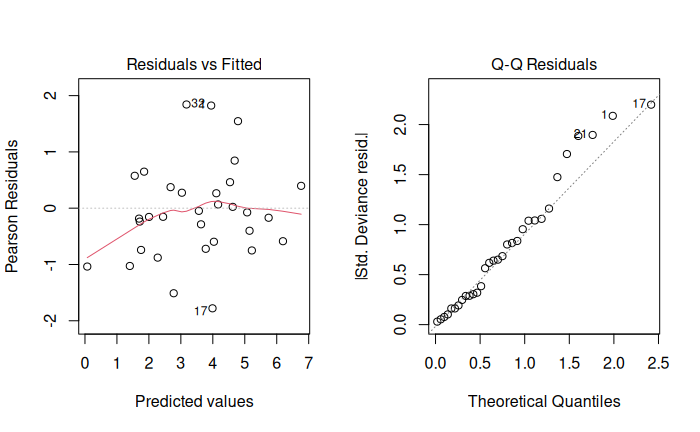
\includegraphics[width=\textwidth]{Images/modelo-poisson-seguros.png}
        \caption{Diagnóstico de residuos (m1).}
        \label{fig:img_top}
    \end{subfigure}
    
    \vspace{0.5cm} % Espacio vertical entre las imágenes
    
    % --- Imagen Inferior ---
    \begin{subfigure}[b]{0.8\textwidth} % Ancho de la subfigura
        \centering
        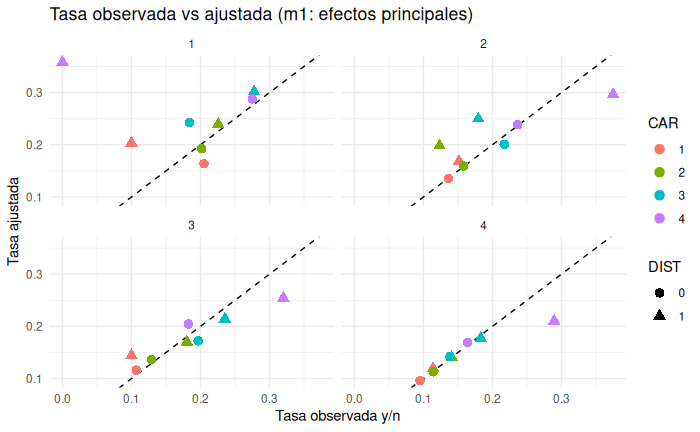
\includegraphics[width=\textwidth]{Images/tasa-obs-vs-ajustada-poisson-seguros.png}
        \caption{Tasa observada vs. ajustada (m1).}
        \label{fig:img_bottom}
    \end{subfigure}
    
    \caption{Resultados del GLM Poisson.}
    \label{fig:matriz_vertical}
\end{figure}




%%%%%%%%%%%%%%%%%%%%%%%%%%%%%%%%%%%%%%%%%%%%%%%%%%%%%%%%%%%%%%%%%%%%%%%%%%%%%
%%%%%%%%%%%%%%%%%%%%%%%%%%%%%%%%%%%%%%%%%%%%%%%%%%%%%%%%%%%%%%%%%%%%%%%%%%%%%

\begin{myblock}
    
    \textbf{(c)} Usando la normalidad asintótica de los estimadores de máxima verosimlitud, da un 
     intervalo del 90\% de confianza para la diferencia en medias. Hay evidencia de diferencias en los
     dos grupos en cuanto a las medias de los conteos?
\end{myblock}

Sea $y_g \sim \text{Poisson}(n_g\lambda_g)$ para $g \in \{0,1\}$ (distritos), con $n_g$ pólizas (exposición) y $\lambda_g$ la tasa por póliza.

El EMV es $\hat{\lambda}_g = y_g/n_g$ y, asintóticamente,
\[
    \operatorname{Var}(\hat{\lambda}_g) \approx \frac{\lambda_g}{n_g} \quad \Rightarrow \quad \widehat{\operatorname{Var}}(\hat{\lambda}_g) \approx \frac{\hat{\lambda}_g}{n_g}.
\]
Para la diferencia de medias $\Delta = \lambda_1 - \lambda_0$,
\[
    \hat{\Delta} = \hat{\lambda}_1 - \hat{\lambda}_0, \qquad \widehat{\operatorname{SE}}(\hat{\Delta}) = \sqrt{\frac{\hat{\lambda}_1}{n_1} + \frac{\hat{\lambda}_0}{n_0}}.
\]
Un IC del 90\% (normal) es
\[
    \hat{\Delta} \pm z_{0.95}\,\widehat{\operatorname{SE}}(\hat{\Delta}), \qquad z_{0.95} = 1.6449.
\]

Sumando por distrito (de la tabla original):
\[
    y_0=2825, \; n_0=21365 \quad \Rightarrow \quad \hat{\lambda}_0=0.13223.
\]
\[
    y_1=326, \; n_1=1994 \quad \Rightarrow \quad \hat{\lambda}_1=0.16349.
\]

Diferencia:
\[
    \hat{\Delta} = 0.16349 - 0.13223 = 0.03126.
\]

Error estándar:
\[
    \widehat{\operatorname{SE}} = \sqrt{\frac{0.16349}{1994} + \frac{0.13223}{21365}} = 0.00939.
\]

IC 90\%:
\[
    0.03126 \pm 1.6449 \times 0.00939 = (0.01582, \; 0.04671).
\]

Por lo tanto, en promedio, \texttt{DIST=1} tiene entre 1.6 y 4.7 reclamos adicionales por cada 100 pólizas,
respecto a \texttt{DIST=0}. El intervalo no incluye a 0, por lo que hay evidencia de que existe diferencia
en las medias de los conteos entre distritos al 90\%. Esto, a su vez, es coherente con lo encontrado
por el IRR > 1 del inciso anterior. 



%%%%%%%%%%%%%%%%%%%%%%%%%%%%%%%%%%%%%%%%%%%%%%%%%%%%%%%%%%%%%%%%%%%%%%%%%%%%%
%%%%%%%%%%%%%%%%%%%%%%%%%%%%%%%%%%%%%%%%%%%%%%%%%%%%%%%%%%%%%%%%%%%%%%%%%%%%%




%%%%%%%%%%%%%%%%%%%%%%%%%%%%%%%%%%%%%%%%%%%%%%%%%%%%%%%%%%%%%%%%%%%%%%%%%%%%%
%%%%%%%%%%%%%%%%%%%%%%%%%%%%%%%%%%%%%%%%%%%%%%%%%%%%%%%%%%%%%%%%%%%%%%%%%%%%%






%\subsection{Teoría}

%\subsection{Resumen de código}

%\subsection{Resultados}

%\subsection{Conclusiones}

\clearpage
\newpage
%%%%%%%%%%%%%%%%%%%%%%%%%%%%%%%%%%%%%%%%%%%%%%%%%%%%%%%%%%%%%%%%
%%%%%%%%%%%%%%%%%%%%%%%%%%%%%%%%%%%%%%%%%%%%%%%%%%%%%%%%%%%%%%%%
%%%%%%%%%%%%%%%%%%%%%%%%%% Enunciado %%%%%%%%%%%%%%%%%%%%%%%%%%%

\begin{myblock}
\phantomsection\addcontentsline{toc}{section}{Ejercicio \#8 | Estimación por Mínima Ji-Cuadrada}
\section*{Ejercicio \#8 | Estimación por Mínima Ji-Cuadrada}

El objetivo de este problema es estimar las proporciones $\pi_1, \pi_2$ y $\pi_3$ correspondientes a tres categorías de objetos (A, B y C) en una población. En lugar de utilizar el método de máxima verosimilitude, se empleará el método de la \textbf{mínima ji-cuadrada}. Este consiste en encontrar los valores de los parámetros que minimizan el estadístico de Pearson ($\chi^2$).

Los datos provienen de un diseño de muestreo particular en el que se tomaron tres muestras independientes para registrar la frecuencia de una sola categoría en cada una:
\begin{itemize}
    \item Número de objetos 'A' en una muestra de tamaño $n_1=100$: $y_1=22$.
    \item Número de objetos 'B' en una muestra de tamaño $n_2=150$: $y_2=52$.
    \item Número de objetos 'C' en una muestra de tamaño $n_3=200$: $y_3=77$.
\end{itemize}

El estadístico de Pearson a minimizar se construye sumando los componentes de cada muestra, donde cada una se considera un ensayo binomial (ej. 'A' vs 'no A'). La función objetivo a minimizar para encontrar $\pi_1, \pi_2$ y $\pi_3$ es:
\[
    \chi^2 = \sum_{i=1}^{3} \left[ \frac{(y_i - n_i\pi_i)^2}{n_i\pi_i} + \frac{((n_i-y_i) - n_i(1-\pi_i))^2}{n_i(1-\pi_i)} \right]
\]
La estimación está sujeta a la restricción $ \pi_1 + \pi_2 + \pi_3 = 1 $. Se sugiere resolver este problema de optimización numérica utilizando la función \texttt{nlminb} de R.

\end{myblock}

%%%%%%%%%%%%%%%%%%%%%%%%%%%%%%%%%%%%%%%%%%%%%%%%%%%%%%%%%%%%%%%%
%%%%%%%%%%%%%%%%%%%%%%%%%%%%%%%%%%%%%%%%%%%%%%%%%%%%%%%%%%%%%%%%

%%%%%%%%%%%%%%%%%%%%%%%%%%%%%%%%%%%%%%%%%%%%%%%%%%%%%%%%%%%%%%%%
%%%%%%%%%%%%%%%%%%%%%%%%%%%%%%%%%%%%%%%%%%%%%%%%%%%%%%%%%%%%%%%%

\subsection{Teoría}

Queremos estimar las proporciones de una multinomial de tres categorías:

\[
    \pi = (\pi_1, \pi_2, \pi_3) \;\;\; \pi_j \leq 0 \;\;\; \pi_1 + \pi_2 + \pi_3 = 1
\]

Normlaemnte, usaríamos máxima verosimilitud (MLE). pero se nos propuso una técnica diferente: utilizar
mínima ji-cuadráda. Esta idea se basa en ajustar las probabilidades de maenra que se minimice el estadístico
de Pearson:

\[
    \chi^2(\pi) = \sum_{j=1}^{K} \frac{(y_j  n \pi_j (\theta))^2}{n \pi_j (\theta)}
\]

En este problema en particular, no tenemos una muestra única multinomial, sino tres estudios independientes
con tamañoa $n_1, n_2, n_3$, y cada uno reporta únicamente la frecuencia de una categoría:

\begin{itemize}
    \item En el estudio número 1 se registró el número de A'S.
    \item En el estudio número 2 el número de B's.
    \item En el estudio número 3 el número de C's.
\end{itemize}

De ese modo, cada muestra aporta información parcial sobre las $\pi_1, \pi_2, \pi_3$. 

Ahora bien, el criterio de mínima ji-cuadrada se construye sumando, para cada estudio, la discrepancia
entre lo observado y lo esperado bajo $\pi$. 

Para la muestra 1 con $(n_1,y_1)$, tenemos:

\[
    \frac{(y_1 - n_1 \pi_1)^2}{n_1 \pi_1} + \frac{((n_1 - y_1) - n_1(1 - \pi_1))^2}{n_1(1 - \pi_1)}
\]

Para la muestra 2 con $(n_2, y_2)$:

\[
    \frac{(y_2 - n_2 \pi_2)^2}{n_2 \pi_2} + \frac{((n_2 - y_2) - n_2(1 - \pi_2))^2}{n_2(1 - \pi_2)}
\]

Para la muestra 3 con $(n_3, y_3)$:

\[
    \frac{(y_3 - n_3 \pi_3)^2}{n_3 \pi_3} + \frac{((n_3 - y_3) - n_3(1 - \pi_3))^2}{n_3(1 - \pi_3)}
\]

Sin embargo, tenemos una restricción. Sabemos que:

\[
    \pi_1 + \pi_2 + \pi_3 = 1 \;\;\; => \;\;\; \pi_3 = 1 - \pi_1 - \pi_2
\]

Esto reduce el problema de tres parámetros a dos libres $(\pi_1, \pi_2)$. 

En resumidas cuenta, lo que debemos resolver es:

\[
    \min_{\pi_1, \pi_2 \geq0, \pi_1 + \pi_2 \leq 1} Q(\pi_1, \pi_2)
\]

Donde: 

\[
\begin{split}
Q(\pi_1, \pi_2) = & \frac{(y_1 - n_1 \pi_1)^2}{n_1 \pi_1} + \frac{((n_1 - y_1) - n_1(1 - \pi_1))^2}{n_1(1 - \pi_1)} \\
& + \frac{(y_2 - n_2 \pi_2)^2}{n_2 \pi_2} + \frac{((n_2 - y_2) - n_2(1 - \pi_2))^2}{n_2(1 - \pi_2)} \\
& + \frac{(y_3 - n_3(1 - \pi_1 - \pi_2))^2}{n_3(1 - \pi_1 - \pi_2)} + \frac{((n_3 - y_3) - n_3(\pi_1 + \pi_2))^2}{n_3(\pi_1 + \pi_2)}
\end{split}
\]

Lo que haremos a continuación será aplicar mínima ji-cuadrada para ajustar una función de pérdida similar
a la de un modelo de regresión multinomial, pero en lugar de maximizar la log-verosimilitud, estamos 
minimizando una suma de discrepancias de $\chi^2$. Es decir, mientras con MLE se aproxima el máximo 
ajuste estadístico, con mínima ji-cuadrada se aproxima al mínimo desajuste respecto a lo esperado. 

\subsection{Resultados}

\begin{table}[h!]
    \centering
    \caption{Resultados de la optimización numérica para las proporciones $\pi_i$ mediante el método de mínima ji-cuadrada, utilizando la función \texttt{nlminb} en R.}
    \label{tab:opt_results}
    \begin{tabular}{lc}
        \toprule
        \textbf{Componente} & \textbf{Valor} \\
        \midrule
        \multicolumn{2}{c}{\textit{Estimaciones de Parámetros}} \\
        $\hat{\pi}_1$ & 0.2395 \\
        $\hat{\pi}_2$ & 0.3629 \\
        $\hat{\pi}_3$ (calculado) & 0.3976 \\
        \midrule
        \multicolumn{2}{c}{\textit{Detalles de la Optimización}} \\
        Valor final del objetivo ($\chi^2$) & 0.5123 \\
        Código de convergencia & 0 (\'Exito) \\
        Mensaje de convergencia & Relative convergence (4) \\
        Iteraciones & 13 \\
        Evaluaciones de la función & 21 \\
        Evaluaciones del gradiente & 38 \\
        \bottomrule
    \end{tabular}
\end{table}

En el cuadro \ref{tab:opt_results}, podemos encontrar los resultados de nuestro intento de optimización. 

Las proporciones observadas por muestra son:

\[
    \frac{y_1}{n_1} = 0.22 \;\;\;\;\; \frac{y_2}{n_2} = 0.3467 \;\;\;\;\; \frac{y_3}{n_3} = 0.385
\]

Al sumarlas, tenemos un aproximado de $ \frac{y_1}{n_1} +  \frac{y_2}{n_2} +  \frac{y_3}{n_3} = 0.9517 < 1$. Es decir,
la restricción impuesta de $\pi_1 + \pi_2 + \pi_3 = 1$ por el modelo multivariado produce \textit{shrinkage}, 
lo cual incrementa ligeramente las estiamciones $\hat{\pi}_m$ respecto a las proporciones en crudo. Este
fenómeno ocurre al minimizar el estadístico de Pearson agregado:

\[
    Q(\pi_1, \pi_2) = \sum_{m=1}^{3} \frac{(y_m - n_m \pi_m)^2}{n_m \pi_m (1 - \pi_m)}
\]

En esta expresión, cada término corresponde a una distribución binomial. La solución equivale a un problema
de optimización con multiplicadores de Lagrange, donde cada $\pi_m$ se ajusta balanceando su
residuo ponderado po rla varianza esperada bajo el modelo. 

Recordemos que tenemos tres muestras binomiales, pero se estimaron dos parámetros libres, tal que tenemos
un $p-value \approx 0.47$. Este resultado no sdice que los datos son compatibles con un único vector 
$\pi$ común a las tres muestras. 

Ahora, revisando los residuos de Pearson, para cada muestra $m$ tenemos:

\[  
    r_m = \frac{y_m - n_m \hat{\pi}_m}{\sqrt{n_m \hat{\pi}_m(1 - \hat{\pi}_m)}} \;\;\;\; r_m^2 \;\; \text{aporta a Q}
\]

\begin{align*}
    \text{Muestra 1: } n_1\hat{\pi}_1 = 23.95, \; y_1=22 & \rightarrow r_1^2 \approx 0.210 \\
    \text{Muestra 2: } n_2\hat{\pi}_2 = 54.43, \; y_2=52 & \rightarrow r_2^2 \approx 0.171 \\
    \text{Muestra 3: } n_3\hat{\pi}_3 = 79.51, \; y_3=77 & \rightarrow r_3^2 \approx 0.137
\end{align*}
Suma $\approx 0.518$ (coincide con $Q \approx 0.512$ por redondeo).

El estimador de mínima ji-cuadrada es asintóticamente equivalente al MLE bajo el modelo correcto.
Aquí resulta muy cercano a resolver el problema de MLE con la restricción lineal 
$\pi_1 + \pi_2 + \pi_3 = 1$. Por tanto, es razonable usar estas $\hat{\pi}$ como 
estimaciones puntuales y construir IC's mediante la matriz de información observada 
(Hessiano) o bootstrap paramétrico.

\clearpage
\newpage
%%%%%%%%%%%%%%%%%%%%%%%%%%%%%%%%%%%%%%%%%%%%%%%%%%%%%%%%%%%%%%%%
%%%%%%%%%%%%%%%%%%%%%%%%%%%%%%%%%%%%%%%%%%%%%%%%%%%%%%%%%%%%%%%%
%%%%%%%%%%%%%%%%%%%%%%%%%% Enunciado %%%%%%%%%%%%%%%%%%%%%%%%%%%

\begin{myblock}
\phantomsection\addcontentsline{toc}{section}{Ejercicio \#9 | Modelo log-lineal para el dataset Titanic}
\section*{Ejercicio \#9 | Modelo log-lineal para el dataset Titanic}

Este problema analiza los datos históricos del hundimiento del Titanic en 1912. El objetivo es utilizar un \textbf{modelo log-lineal} para investigar las asociaciones e interacciones entre cuatro variables categóricas que describen a los pasajeros.

Los datos, disponibles en la librería \texttt{titanic} de R, se presentan en una tabla de contingencia de cuatro dimensiones con las siguientes variables:
\begin{itemize}
    \item \textbf{Class}: Clase del pasajero (1, 2, 3, Tripulación).
    \item \textbf{Sex}: Sexo (Male, Female).
    \item \textbf{Age}: Grupo de edad (Child, Adult).
    \item \textbf{Survived}: Estado de supervivencia (No, Yes).
\end{itemize}

Se debe ajustar un modelo log-lineal para evaluar la significancia de los siguientes efectos y así comprender la estructura de dependencias en los datos:
\begin{enumerate}
    \item \textbf{Efectos Principales}: Determinar si las frecuencias de pasajeros son uniformes a través de las categorías de \texttt{Class}, \texttt{Sex}, \texttt{Age} y \texttt{Survived}.
    \item \textbf{Interacciones de Dos Vías}: Evaluar la independencia entre cada par de variables (ej. \texttt{Sex} $\times$ \texttt{Survived}, \texttt{Class} $\times$ \texttt{Age}).
    \item \textbf{Interacciones de Orden Superior}: Investigar las dependencias más complejas, incluyendo todas las interacciones de tres vías y la interacción de cuatro vías.
\end{enumerate}

\end{myblock}

%%%%%%%%%%%%%%%%%%%%%%%%%%%%%%%%%%%%%%%%%%%%%%%%%%%%%%%%%%%%%%%%
%%%%%%%%%%%%%%%%%%%%%%%%%%%%%%%%%%%%%%%%%%%%%%%%%%%%%%%%%%%%%%%%

%%%%%%%%%%%%%%%%%%%%%%%%%%%%%%%%%%%%%%%%%%%%%%%%%%%%%%%%%%%%%%%%
%%%%%%%%%%%%%%%%%%%%%%%%%%%%%%%%%%%%%%%%%%%%%%%%%%%%%%%%%%%%%%%%

Para lograr investigar el comportamiento de independencia entre variables categóricas de estudio, implementamos
un modelo log-lineal jerárquico. Este enfoque permite evaluar de manera sistemática la contribución de interacciones
de creciente complejidad para explicar las frecuencias observadas en la tabla de contingencia. Se compararon cuatro
modelos anidados, cada uno representando una hipótesis específica sobre la relación entre las variables.

La selección del modelo óptimo se basó en el estadístico de razón de verosimilitud que compara el ajuste
de cad amoedlo propuesto con el ajuste del modelo saturado. Los modelos evaluados fueron:

\begin{itemize}
    \item \textbf{Modelo de Independencia Total (m0):} Este modelo base postula que no existe asociaci\'{o}n alguna entre ninguna de las variables. Matem\'{a}ticamente, se expresa como:
    $$ \log E[n_{ijkl}] = \mu + \alpha_i + \beta_j + \gamma_k + \delta_l $$
    La evaluaci\'{o}n de este modelo arroj\'{o} un ajuste extremadamente deficiente ($G^2 = 1243.66$ con 25 grados de libertad, $p \approx 0$). Este resultado permite rechazar de forma contundente la hip\'{o}tesis de que las variables son mutuamente independientes.

    \item \textbf{Modelo de Interacciones de Dos Vías (m2):} El segundo modelo incorpora todas las posibles asociaciones por pares entre las variables. Aunque represent\'{o} una mejora sustancial respecto al modelo de independencia, su ajuste segu\'{\i}a siendo estad\'{\i}sticamente inadecuado ($G^2 = 116.59$ con 13 grados de libertad, $p \approx 0$). Esto indica que las meras asociaciones entre pares de variables no son suficientes para capturar la complejidad de la estructura subyacente en los datos.

    \item \textbf{Modelo de Interacciones de Tres Vías (m3):} Este modelo representa el punto de inflexi\'{o}n en nuestro an\'{a}lisis. Al incluir todos los t\'{e}rminos de interacci\'{o}n de tres v\'{\i}as (y, por el principio de jerarqu\'{\i}a, los t\'{e}rminos de orden inferior), el modelo present\'{o} un ajuste excepcional a los datos observados ($G^2 = 2.73 \times 10^{-4}$ con 3 grados de libertad, $p \approx 0.999999$). Un valor de devianza pr\'{a}cticamente nulo y un p-valor cercano a 1 constituyen una fuerte evidencia de que este modelo explica casi la totalidad de la estructura de dependencia presente.

    \item \textbf{Modelo Saturado (m4):} Este modelo, que incluye la interacci\'{o}n de cuatro v\'{\i}as, reproduce perfectamente los datos por definici\'{o}n ($G^2 = 0$ con 0 grados de libertad). No aporta informaci\'{o}n explicativa adicional, pero sirve como referencia para confirmar que el modelo m3 ya ha capturado toda la estructura de dependencia relevante.
\end{itemize}

De ese modo, la evidencia estadística nos está diciendo que describir adecuadamente las relaciones enter variables
es indispensable incluir los términos de interacción de tres vías. El modelo $m3$ es la más precisa 
con la estructura de los datos. A su vez, la necesiadd de un término de interacción de tres vías implica
que la relación entre dos variables cualesquiera no es constante, sin oque stá moderada o condicionada 
por el valor ed una tercera variable. 

El efecto del Sexo sobre la Supervivencia no es el mismo en todas las Clases o para todos los grupos de Edad.
De manera an\'{a}loga, el impacto de la Edad en la probabilidad de Supervivencia se ve modificado por la Clase del individuo y su Sexo.
En esencia, la narrativa popular de ``mujeres y ni\~{n}os primero'' no fue un protocolo aplicado de manera uniforme. Su implementaci\'{o}n y, por tanto, la probabilidad de supervivencia, dependi\'{o} de manera crucial de la clase social a la que pertenec\'{i}an los individuos, revelando una interacci\'{o}n compleja y de orden superior.

Durante el an\'{a}lisis, se observ\'{o} que el estad\'{\i}stico chi-cuadrado de Pearson arrojaba un valor no definido (\texttt{NaN}). Esto se debe a la presencia de ceros estructurales en la tabla de contingencia (por ejemplo, la combinaci\'{o}n ``Tripulaci\'{o}n-Ni\~{n}o'' es l\'{o}gicamente imposible y su frecuencia observada es cero). En ciertos modelos, esto induce frecuencias esperadas ($E$) nulas para dichas celdas. Dado que el c\'{a}lculo del estad\'{\i}stico de Pearson implica una divisi\'{o}n por $E$ ($\sum \frac{(O-E)^2}{E}$), la presencia de un cero en el denominador provoca una indeterminaci\'{o}n matem\'{a}tica.

Por esta raz\'{o}n, el estad\'{\i}stico de raz\'{o}n de verosimilitud ($G^2$) es el m\'{e}todo preferido y m\'{a}s robusto para el an\'{a}lisis de tablas de contingencia que contienen ceros estructurales, ya que su c\'{a}lculo no presenta esta limitaci\'{o}n.

\clearpage
\newpage
%%%%%%%%%%%%%%%%%%%%%%%%%%%%%%%%%%%%%%%%%%%%%%%%%%%%%%%%%%%%%%%%
%%%%%%%%%%%%%%%%%%%%%%%%%%%%%%%%%%%%%%%%%%%%%%%%%%%%%%%%%%%%%%%%
%%%%%%%%%%%%%%%%%%%%%%%%%% Enunciado %%%%%%%%%%%%%%%%%%%%%%%%%%%

\begin{myblock}
\phantomsection\addcontentsline{toc}{section}{Ejercicio \#10 | Descripción del corpus}
\section*{Ejercicio \#10 | Descripción del corpus}

Se ha realizado un análisis sobre el valor terapéutico del ácido ascórbico (Vitamina C) en relación
a su efecto sobre la gripe común. Se tiene una tabla $2 \times 2$ con los recuentos
correspondientes para una muestra de 279 personas.

Aplica un modelo lineal para determinar si existe ecvidencia suficiente para asgurar que el ácido 
ascorbico ayuda a tener menos gripe. 

\end{myblock}

%%%%%%%%%%%%%%%%%%%%%%%%%%%%%%%%%%%%%%%%%%%%%%%%%%%%%%%%%%%%%%%%
%%%%%%%%%%%%%%%%%%%%%%%%%%%%%%%%%%%%%%%%%%%%%%%%%%%%%%%%%%%%%%%%

\begin{table}[h!]
\centering
\caption{Tabla de contingencia del estudio sobre el Ácido Ascórbico.}
\label{tab:gripe}
\begin{tabular}{l|cc|c}
\multicolumn{1}{c}{} & \textbf{Gripe} & \textbf{No Gripe} & \textit{Totales} \\
\hline
Placebo             & 31 & 109 & 140 \\
Acido Asc\'{o}rbico & 17 & 122 & 139 \\
\hline
\textit{Totales}    & 48 & 231 & 279 \\
\end{tabular}
\end{table}

%%%%%%%%%%%%%%%%%%%%%%%%%%%%%%%%%%%%%%%%%%%%%%%%%%%%%%%%%%%%%%%%
%%%%%%%%%%%%%%%%%%%%%%%%%%%%%%%%%%%%%%%%%%%%%%%%%%%%%%%%%%%%%%%%

\begin{figure}[h!]
    \centering
    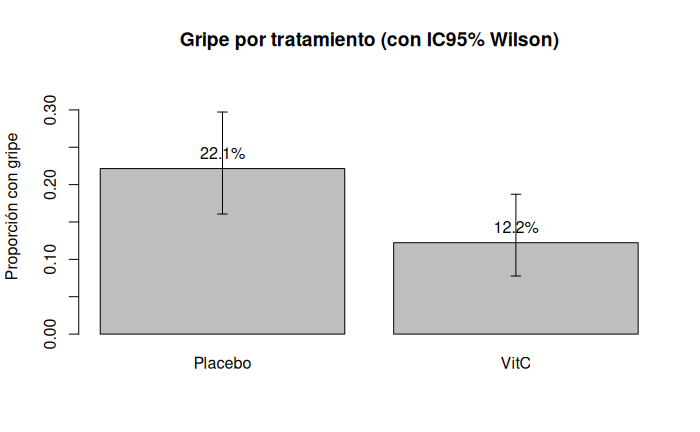
\includegraphics[width=0.7\linewidth]{Images/gripe-p10.png}
    \caption{Gripe GLM.}
    \label{fig:gripe-10}
\end{figure}


Se evaluó el efecto terapéutico del ácido ascórbico (Vitamina C) sobre la incidencia de gripe en un ensayo con $n=279$ personas, asignadas a los grupos de Placebo ($n=140$) y Vitamina C ($n=139$). La respuesta considerada fue binaria: presencia o ausencia de gripe. La tabla de contingencia observada fue: Placebo con 31 casos de gripe y 109 sin gripe, y Vitamina C con 17 casos de gripe y 122 sin gripe. En total se observaron 48 casos de gripe y 231 individuos sanos.

Para el análisis se ajustó un modelo lineal generalizado binomial con enlace logit de la forma
\[
\log \frac{\Pr(Y=1 \mid T)}{1 - \Pr(Y=1 \mid T)} = \beta_0 + \beta_1 \,\mathbb{1}\{T=\text{VitC}\},
\]
donde $Y$ indica la ocurrencia de gripe y $T$ el tratamiento recibido. El interés radica en contrastar la hipótesis unilateral de que $\beta_1 < 0$, es decir, que la administración de Vitamina C reduce la probabilidad de presentar gripe en comparación con el placebo. 

Los resultados del modelo muestran un intercepto estimado de $\hat\beta_0=-1.257$ (SE=0.204), correspondiente al log-odds de gripe en el grupo Placebo, y un coeficiente de tratamiento $\hat\beta_1=-0.713$ (SE=0.329). La odds ratio estimada de Vitamina C respecto a Placebo es $\widehat{\text{OR}}=\exp(\hat\beta_1)=0.490$, con un intervalo de confianza del 95\% dado por $[0.257,\,0.934]$. Esto indica que las odds de gripe con Vitamina C son aproximadamente 51\% menores que con Placebo. La prueba de Wald bilateral produce un valor-$p=0.030$, mientras que en la dirección unilateral favorable a Vitamina C se obtiene $p=0.015$, lo que proporciona evidencia a favor del efecto protector.

Se aplicaron pruebas adicionales de independencia para verificar la robustez del resultado. La prueba de $\chi^2$ de Pearson entrega un estadístico $X^2=4.81$ con un valor-$p=0.028$, lo cual sugiere asociación entre el tratamiento y la incidencia de gripe. Por su parte, la prueba exacta de Fisher unilateral, especificando la hipótesis de que Placebo presenta mayor odds de gripe que Vitamina C, arroja un valor-$p=0.0205$ y un intervalo de confianza unilat. al 95\% de $[1.13,\,\infty)$ para la odds ratio en la escala Placebo vs Vitamina C, equivalente a concluir que la odds ratio Vitamina C vs Placebo es menor que 1. Así, las tres pruebas son consistentes en apoyar la hipótesis de interés.

En términos de riesgos absolutos, la proporción de gripe en el grupo Placebo fue de $\hat p_{\text{Placebo}}=31/140=0.221$, mientras que en el grupo Vitamina C fue de $\hat p_{\text{VitC}}=17/139=0.122$. La reducción absoluta del riesgo estimada es $\hat p_{\text{VitC}} - \hat p_{\text{Placebo}} = -0.099$, es decir, una disminución de 9.9 puntos porcentuales. El riesgo relativo estimado es $\widehat{\text{RR}} = 0.552$, lo cual implica que el riesgo de gripe con Vitamina C es aproximadamente 45\% menor que con Placebo. Finalmente, el número necesario a tratar (NNT) se aproxima como $1/0.099 \approx 10$, interpretándose que, bajo condiciones similares, se deberían tratar 10 personas con Vitamina C para evitar un caso adicional de gripe.

En conclusión, la evidencia estadística proveniente del modelo logístico, la prueba de Pearson y la prueba exacta de Fisher unilateral apoya de manera consistente que el ácido ascórbico reduce la incidencia de gripe en comparación con placebo. La magnitud del efecto es clínicamente relevante, con un odds ratio estimado de 0.49, un riesgo relativo de 0.55, una reducción absoluta del riesgo cercana al 10\% y un número necesario a tratar de alrededor de 10. Estos resultados constituyen un respaldo empírico a la hipótesis de que la Vitamina C ejerce un efecto protector frente a la gripe común.

\clearpage
%\newpage
%%%%%%%%%%%%%%%%%%%%%%%%%%%%%%%%%%%%%%%%%%%%%%%%%%%%%%%%%%%%%%%%
%%%%%%%%%%%%%%%%%%%%%%%%%%%%%%%%%%%%%%%%%%%%%%%%%%%%%%%%%%%%%%%%
%%%%%%%%%%%%%%%%%%%%%%%%%% Enunciado %%%%%%%%%%%%%%%%%%%%%%%%%%%

\begin{myblock}
\phantomsection\addcontentsline{toc}{section}{Ejercicio \#1 | Descripción del corpus}
\section*{Ejercicio \#1 | Descripción del corpus}

Analiza el corpus y reporta:\\

\begin{itemize}
    \item Número de documentos, tokens y vocabulario.
    \item Hapax legomena y su proporción.
    \item Porcentaje y su proporción.
    \item Estadísticas por clase (número de documentos, tokens y vocabulario).
\end{itemize}

\end{myblock}

%%%%%%%%%%%%%%%%%%%%%%%%%%%%%%%%%%%%%%%%%%%%%%%%%%%%%%%%%%%%%%%%
%%%%%%%%%%%%%%%%%%%%%%%%%%%%%%%%%%%%%%%%%%%%%%%%%%%%%%%%%%%%%%%%

%%%%%%%%%%%%%%%%%%%%%%%%%%%%%%%%%%%%%%%%%%%%%%%%%%%%%%%%%%%%%%%%
%%%%%%%%%%%%%%%%%%%%%%%%%%%%%%%%%%%%%%%%%%%%%%%%%%%%%%%%%%%%%%%%

\subsection{Teoría}\\

\subsection{Resumen de código}\\

\subsection{Resultados}\\

\subsection{Conclusiones}\\

\clearpage
%\newpage
%%%%%%%%%%%%%%%%%%%%%%%%%%%%%%%%%%%%%%%%%%%%%%%%%%%%%%%%%%%%%%%%
%%%%%%%%%%%%%%%%%%%%%%%%%%%%%%%%%%%%%%%%%%%%%%%%%%%%%%%%%%%%%%%%
%%%%%%%%%%%%%%%%%%%%%%%%%% Enunciado %%%%%%%%%%%%%%%%%%%%%%%%%%%

\begin{myblock}
\phantomsection\addcontentsline{toc}{section}{Ejercicio \#1 | Descripción del corpus}
\section*{Ejercicio \#1 | Descripción del corpus}

Analiza el corpus y reporta:\\

\begin{itemize}
    \item Número de documentos, tokens y vocabulario.
    \item Hapax legomena y su proporción.
    \item Porcentaje y su proporción.
    \item Estadísticas por clase (número de documentos, tokens y vocabulario).
\end{itemize}

\end{myblock}

%%%%%%%%%%%%%%%%%%%%%%%%%%%%%%%%%%%%%%%%%%%%%%%%%%%%%%%%%%%%%%%%
%%%%%%%%%%%%%%%%%%%%%%%%%%%%%%%%%%%%%%%%%%%%%%%%%%%%%%%%%%%%%%%%

%%%%%%%%%%%%%%%%%%%%%%%%%%%%%%%%%%%%%%%%%%%%%%%%%%%%%%%%%%%%%%%%
%%%%%%%%%%%%%%%%%%%%%%%%%%%%%%%%%%%%%%%%%%%%%%%%%%%%%%%%%%%%%%%%

\subsection{Teoría}\\

\subsection{Resumen de código}\\

\subsection{Resultados}\\

\subsection{Conclusiones}\\

\clearpage
%\newpage
%%%%%%%%%%%%%%%%%%%%%%%%%%%%%%%%%%%%%%%%%%%%%%%%%%%%%%%%%%%%%%%%
%%%%%%%%%%%%%%%%%%%%%%%%%%%%%%%%%%%%%%%%%%%%%%%%%%%%%%%%%%%%%%%%
%%%%%%%%%%%%%%%%%%%%%%%%%% Enunciado %%%%%%%%%%%%%%%%%%%%%%%%%%%

\begin{myblock}
\phantomsection\addcontentsline{toc}{section}{Ejercicio \#1 | Descripción del corpus}
\section*{Ejercicio \#1 | Descripción del corpus}

Analiza el corpus y reporta:\\

\begin{itemize}
    \item Número de documentos, tokens y vocabulario.
    \item Hapax legomena y su proporción.
    \item Porcentaje y su proporción.
    \item Estadísticas por clase (número de documentos, tokens y vocabulario).
\end{itemize}

\end{myblock}

%%%%%%%%%%%%%%%%%%%%%%%%%%%%%%%%%%%%%%%%%%%%%%%%%%%%%%%%%%%%%%%%
%%%%%%%%%%%%%%%%%%%%%%%%%%%%%%%%%%%%%%%%%%%%%%%%%%%%%%%%%%%%%%%%

\subsection{Teoría}\\

\subsection{Resumen de código}\\

\subsection{Resultados}\\

\subsection{Conclusiones}\\

\clearpage

\end{document}
